\documentclass[12pt]{article}
\usepackage{graphicx}
\usepackage[english]{babel}
\usepackage{pdfpages}
\usepackage{caption}
\usepackage{subcaption}
\usepackage[utf8]{inputenc}
\usepackage[sc]{mathpazo} % Use the Palatino font
\usepackage[T1]{fontenc} % Use 8-bit encoding that has 256 glyphs
\linespread{1.05} % Line spacing - Palatino needs more space between lines
%\usepackage{microtype} % Slightly tweak font spacing for aesthetics
%\usepackage[hmarginratio=1:1,top=32mm,columnsep=20pt]{geometry} % Document margins
%\usepackage[hang, small,labelfont=bf,up,textfont=it,up]{caption} % Custom captions under/above floats in tables or figures
%\usepackage{booktabs} % Horizontal rules in tables
%\usepackage{lettrine} % The lettrine is the first enlarged letter at the beginning of the text
%\usepackage{enumitem} % Customized lists
%\setlist[itemize]{noitemsep} % Make itemize lists more compact
%\usepackage{abstract} % Allows abstract customization
%\renewcommand{\abstractnamefont}{\normalfont\bfseries} % Set the "Abstract" text to bold
%\renewcommand{\abstracttextfont}{\normalfont\small\itshape} % Set the abstract itself to small italic text
\usepackage{esdiff}
\usepackage{titlesec} % Allows customization of titles
\renewcommand\thesection{\Roman{section}} % Roman numerals for the sections
\renewcommand\thesubsection{\roman{subsection}} % roman numerals for subsections
\titleformat{\section}[block]{\large\scshape\centering}{\thesection.}{1em}{} % Change the look of the section titles
\titleformat{\subsection}[block]{\large}{\thesubsection.}{1em}{} % Change the look of the section titles

\usepackage{geometry}
\usepackage{listings}
\usepackage{color}
%\usepackage[usenames,dvipsnames,svgnames,table]{xcolor}
\usepackage{xcolor}
\geometry{a4paper}
    \lstset{
    language=python,
    tabsize=1,
    %frame=lines,
    label=code:sample,
    frame=shadowbox,
    rulesepcolor=\color{gray},
    xleftmargin=+5pt,
    framexleftmargin=25pt,
    xrightmargin = -25pt,
    keywordstyle=\color{blue}\bf,
    commentstyle=\color{green},
    stringstyle=\color{red},
    numbers=left,
    numberstyle=\tiny,
    numbersep=5pt,
    breaklines=true,
    showstringspaces=false,
    basicstyle=\footnotesize,
    emph={str},emphstyle={\color{magenta}}}


%\usepackage{fancyhdr} % Headers and footers
%\pagestyle{fancy} % All pages have headers and footers
%\fancyhead{} % Blank out the default header
%\fancyfoot{} % Blank out the default footer
%\fancyhead[C]{Running title $\bullet$ May 2016 $\bullet$ Vol. XXI, No. 1} % Custom header text
%\fancyfoot[RO,LE]{\thepage} % Custom footer text




\usepackage{titling} % Customizing the title section
\usepackage{amsmath}
\usepackage{hyperref} % For hyperlinks in the PDF
\usepackage{xcolor}

%\makeatletter
%\def\mathcolor#1#{\@mathcolor{#1}}
%\def\@mathcolor#1#2#3{%
%  \protect\leavevmode
%  \begingroup
%    \color#1{#2}#3%
%  \endgroup
%}
%\makeatother




%----------------------------------------------------------------------------------------
%	TITLE SECTION
%----------------------------------------------------------------------------------------

\setlength{\droptitle}{-4\baselineskip} % Move the title up

\pretitle{\begin{center}\Huge\bfseries} % Article title formatting
\posttitle{\end{center}} % Article title closing formatting
\title{Exercise 2 - Neural Networks} % Article title
\author{%
\textsc{Alexander Bigalke, Arthur Heimbrecht, Robin Rombach}}
\date{\today} % Leave empty to omit a date



%----------------------------------------------------------------------------------------
\clubpenalty=10000
\widowpenalty=10000 
\displaywidowpenalty=10000


\begin{document}
\maketitle
\section{Classification Capacity}
- see attached handwritten notes beginning next page - 
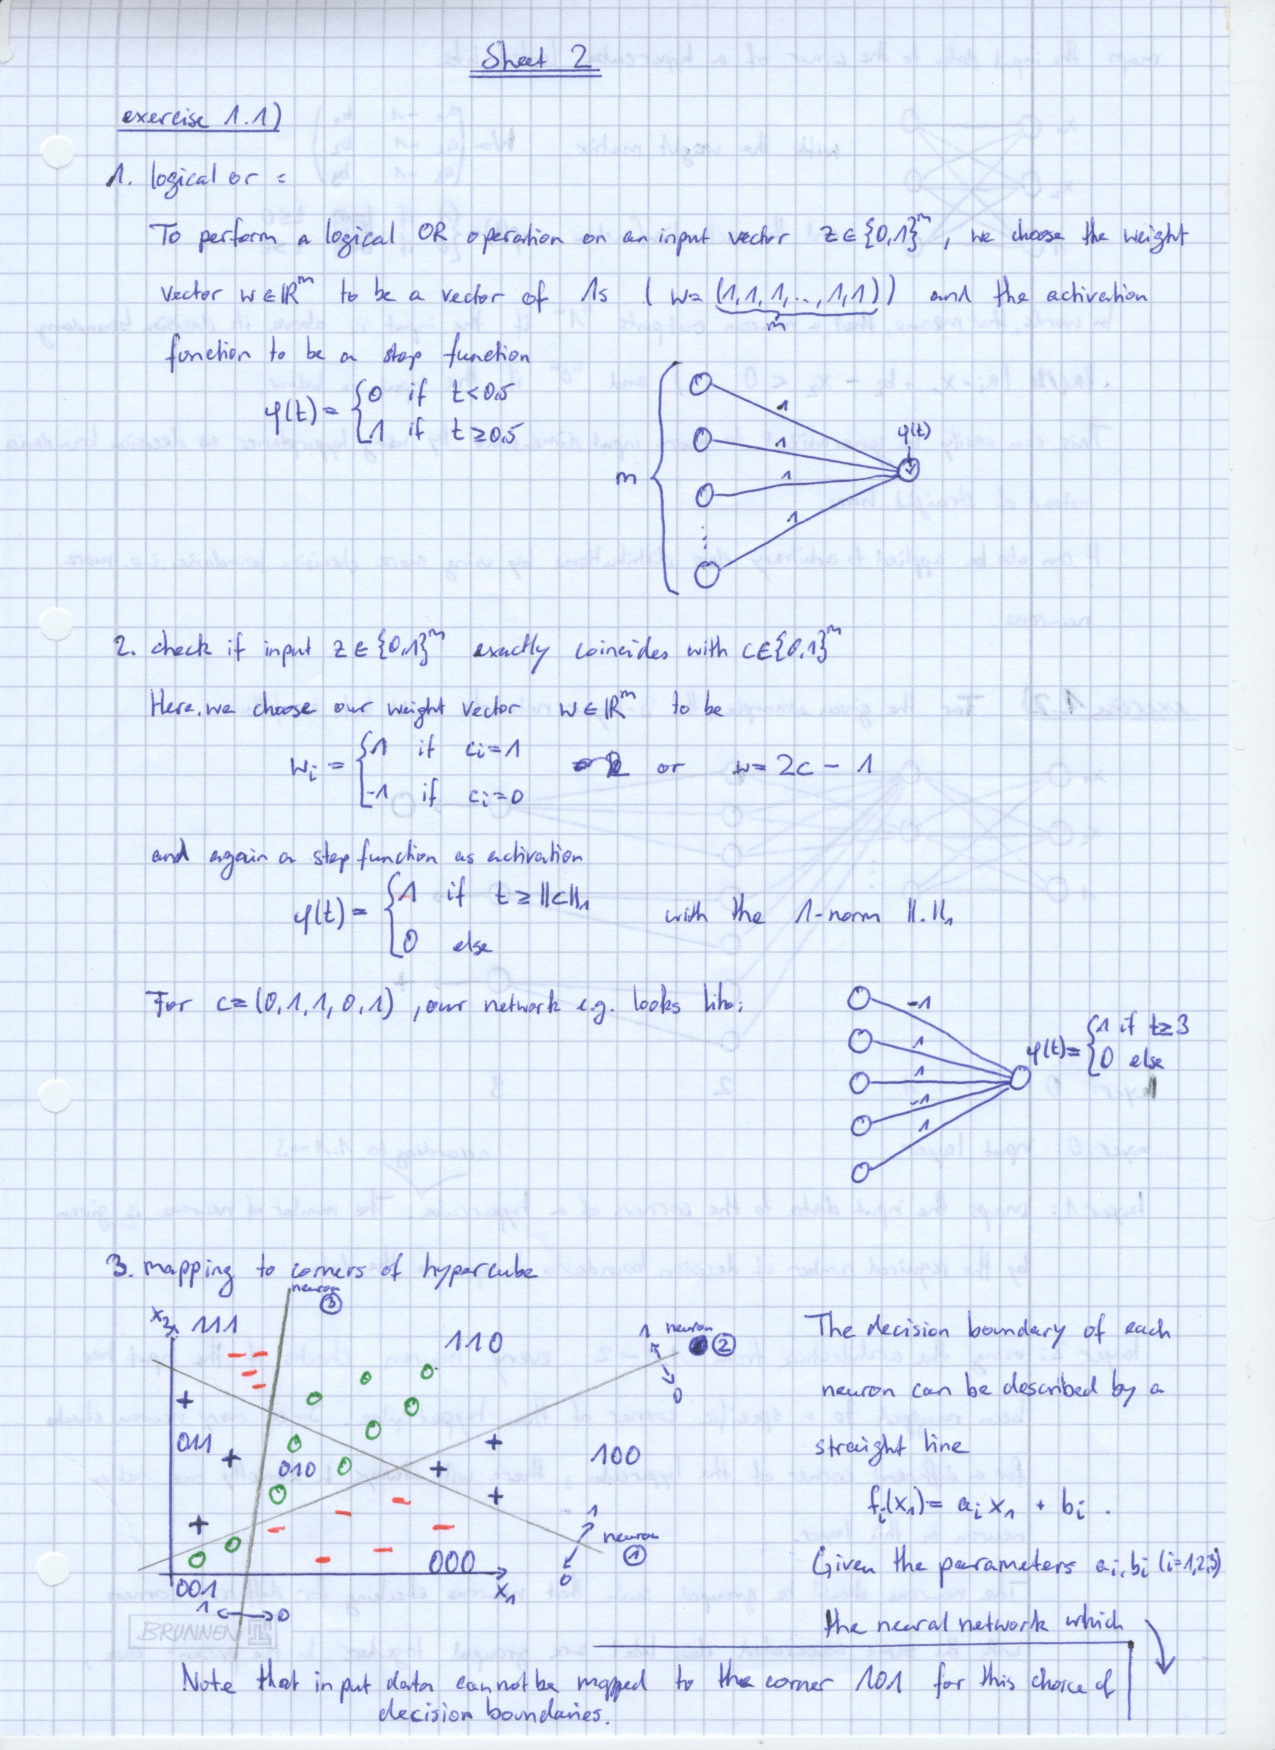
\includepdf[pages=-]{Sheet2_ex1a.pdf}
%\includegraphics{}
\section{Linear Activation Function}
In a feed-forward network, the output of each layer $l$ (denoted $Z_l \; \in \; \mathbb{R}^{m_l}$; with $m_l$ some integer specifying the number of features in layer $l$.) is computed iteratively by multiplying the weight matrix $B_l \; \in \; \mathbb{R}^{m_{l}\times m_{l-1}}$ with the output of layer $l-1$ and subsequently applying the activation function $\varphi_l$ to this product: 
\begin{align}
\tilde{Z}_l &= B_{l} \cdot Z_{l-1} \label{eq:1}\\
Z_l &= \varphi_l(\tilde{Z}_l)
\end{align}
where the input $Z_0$ is given as 
$$ Z_0 = \left( \begin{array}{c}1\\\mathbf{X}\end{array} \right) $$
with $\mathbf{X}$ denoting the input (training) data. \\
\newline
Let us assume that the activation function is a linear map, i.e.
\begin{equation}
Z_l = \varphi_l(\tilde{Z}_l) = \Phi_l \cdot \tilde{Z}_l
\label{eq:3} 
\end{equation} 
such that $\Phi_l$ is a quadratic matrix with $\Phi_l \in \mathbb{R}^{m_l \times m_l}$. \\
Combining equations \eqref{eq:1} and \eqref{eq:3} and exploiting associativity of matrix multiplication then yields the following output for layer $l$:
\begin{equation}
Z_l = \Phi_l \cdot \tilde{Z}_l = \Phi_l \cdot B_l \cdot Z_{l-1} \equiv \mathcal{B}_l \cdot Z_{l-1}\;.
\label{eq:4}
\end{equation}
Hence, $$\mathbb{R}^{m_l \times m_{l-1}}\ni \mathcal{B}_l = \Phi_l \cdot B_l $$
Expanding \eqref{eq:4} gives:
\begin{align}
Z_l = \underbrace{ \mathcal{B}_l \cdot \mathcal{B}_{l-1} \cdot \mathcal{B}_{l-2} \cdot \dots \cdot \mathcal{B}_1}_{\equiv \mathbf{B}_l^0 \: \in \: \mathbb{R}^{m_l \times m_0}} \cdot Z_0 
\label{eq:5}
\end{align}
Thus, in the case of a linear activation function and by contracting the product $\mathcal{B}_l \cdot \mathcal{B}_{l-1} \cdot \mathcal{B}_{l-2} \cdot \dots \cdot \mathcal{B}_1$, the whole procedure of mapping the input layer 0 to layer $l$ via several intermediate layers $l-i$ ($i \; \in \; [0, l]$) reduces to mapping layer 0 directly to layer $l$ by
\begin{equation}
Z_l = \mathbf{B}_l^0 \cdot Z_0
\end{equation}
with $\mathbf{B}_l^0 \: \in \: \mathbb{R}^{m_l \times m_0}$.
\newpage
\enlargethispage{5\baselineskip}
\section{Application}
The completed code can be found in the file \texttt{network.py}. \\ 
\newline
We report results for the following cases: \\
\newline
i) \texttt{layer\_sizes = [2,2, n\_classes]} \\
ii) \texttt{layer\_sizes = [3,3, n\_classes]} \\
iii) \texttt{layer\_sizes = [5,5, n\_classes]} \\
iv) \texttt{layer\_sizes = [30,30, n\_classes]} \\
with \texttt{n\_classes = 2}.\\
\newline
For the other hyper-parameters, we use: \\
\texttt{n\_epochs = 500}; 
\texttt{batch\_size = 200}; 
\texttt{learning\_rate = 0.0001} \\
\newline
The task is to classify a dataset provided by \texttt{sklearn.datasets.make\_moons}. A visualized example-set is provided in Figure \ref{fig:exset}. \\
We account for the stochastic nature of the model (induced by the stochastic gradient descent used here) by repeating each classification run (for a fixed set of hyper-parameters) $n = 10$ times and subsequently computing mean, median and standard deviation of the resulting error rate(s). 
\begin{figure}[hbtp]
\begin{center}
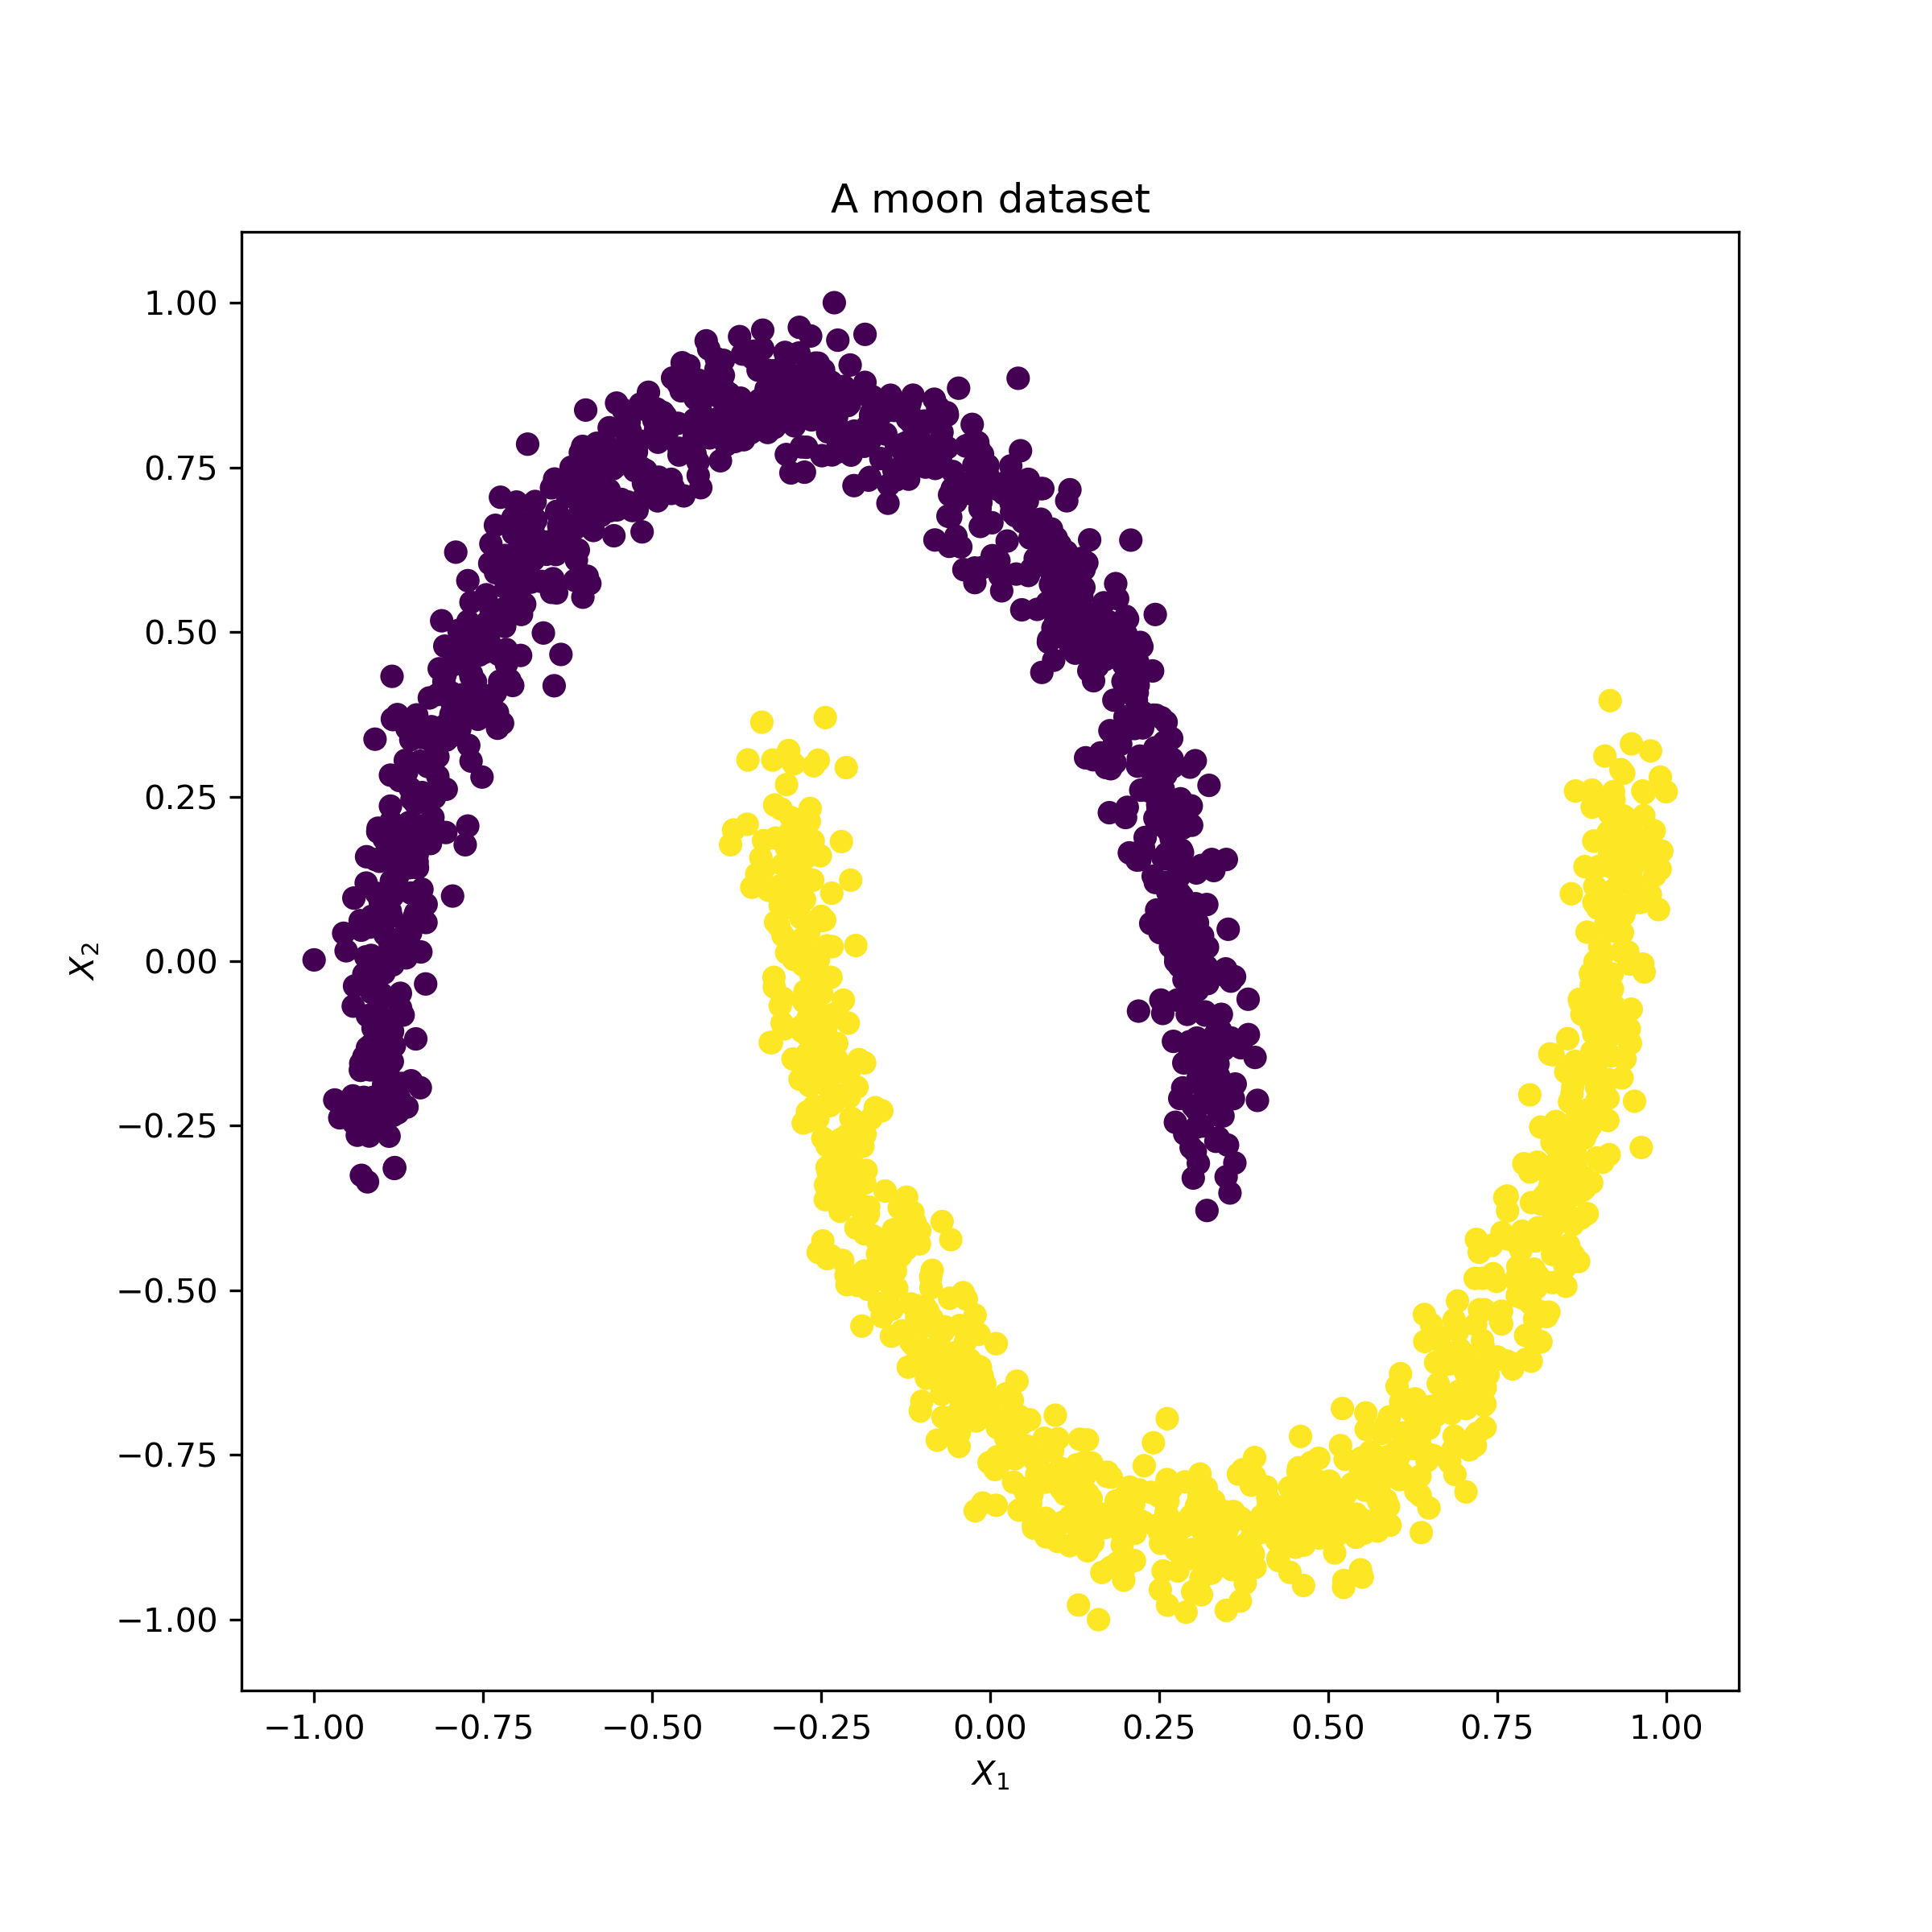
\includegraphics[scale=0.38]{pics/exampleset.png}
\caption{An instance of \texttt{sklearn.datasets.make\_moons} with 2 classes.}
\label{fig:exset}
\end{center}
\end{figure}
\noindent In the following, let $\gamma_t$ denote the error rate on the test set.\\
\newpage
\textbf{i):} \texttt{layer\_sizes = [2,2, n\_classes]} \\
\begin{figure}[htbp]
\captionsetup[subfigure]{labelformat=empty}
\centering
	\begin{subfigure}{.48\textwidth}
	\centering
	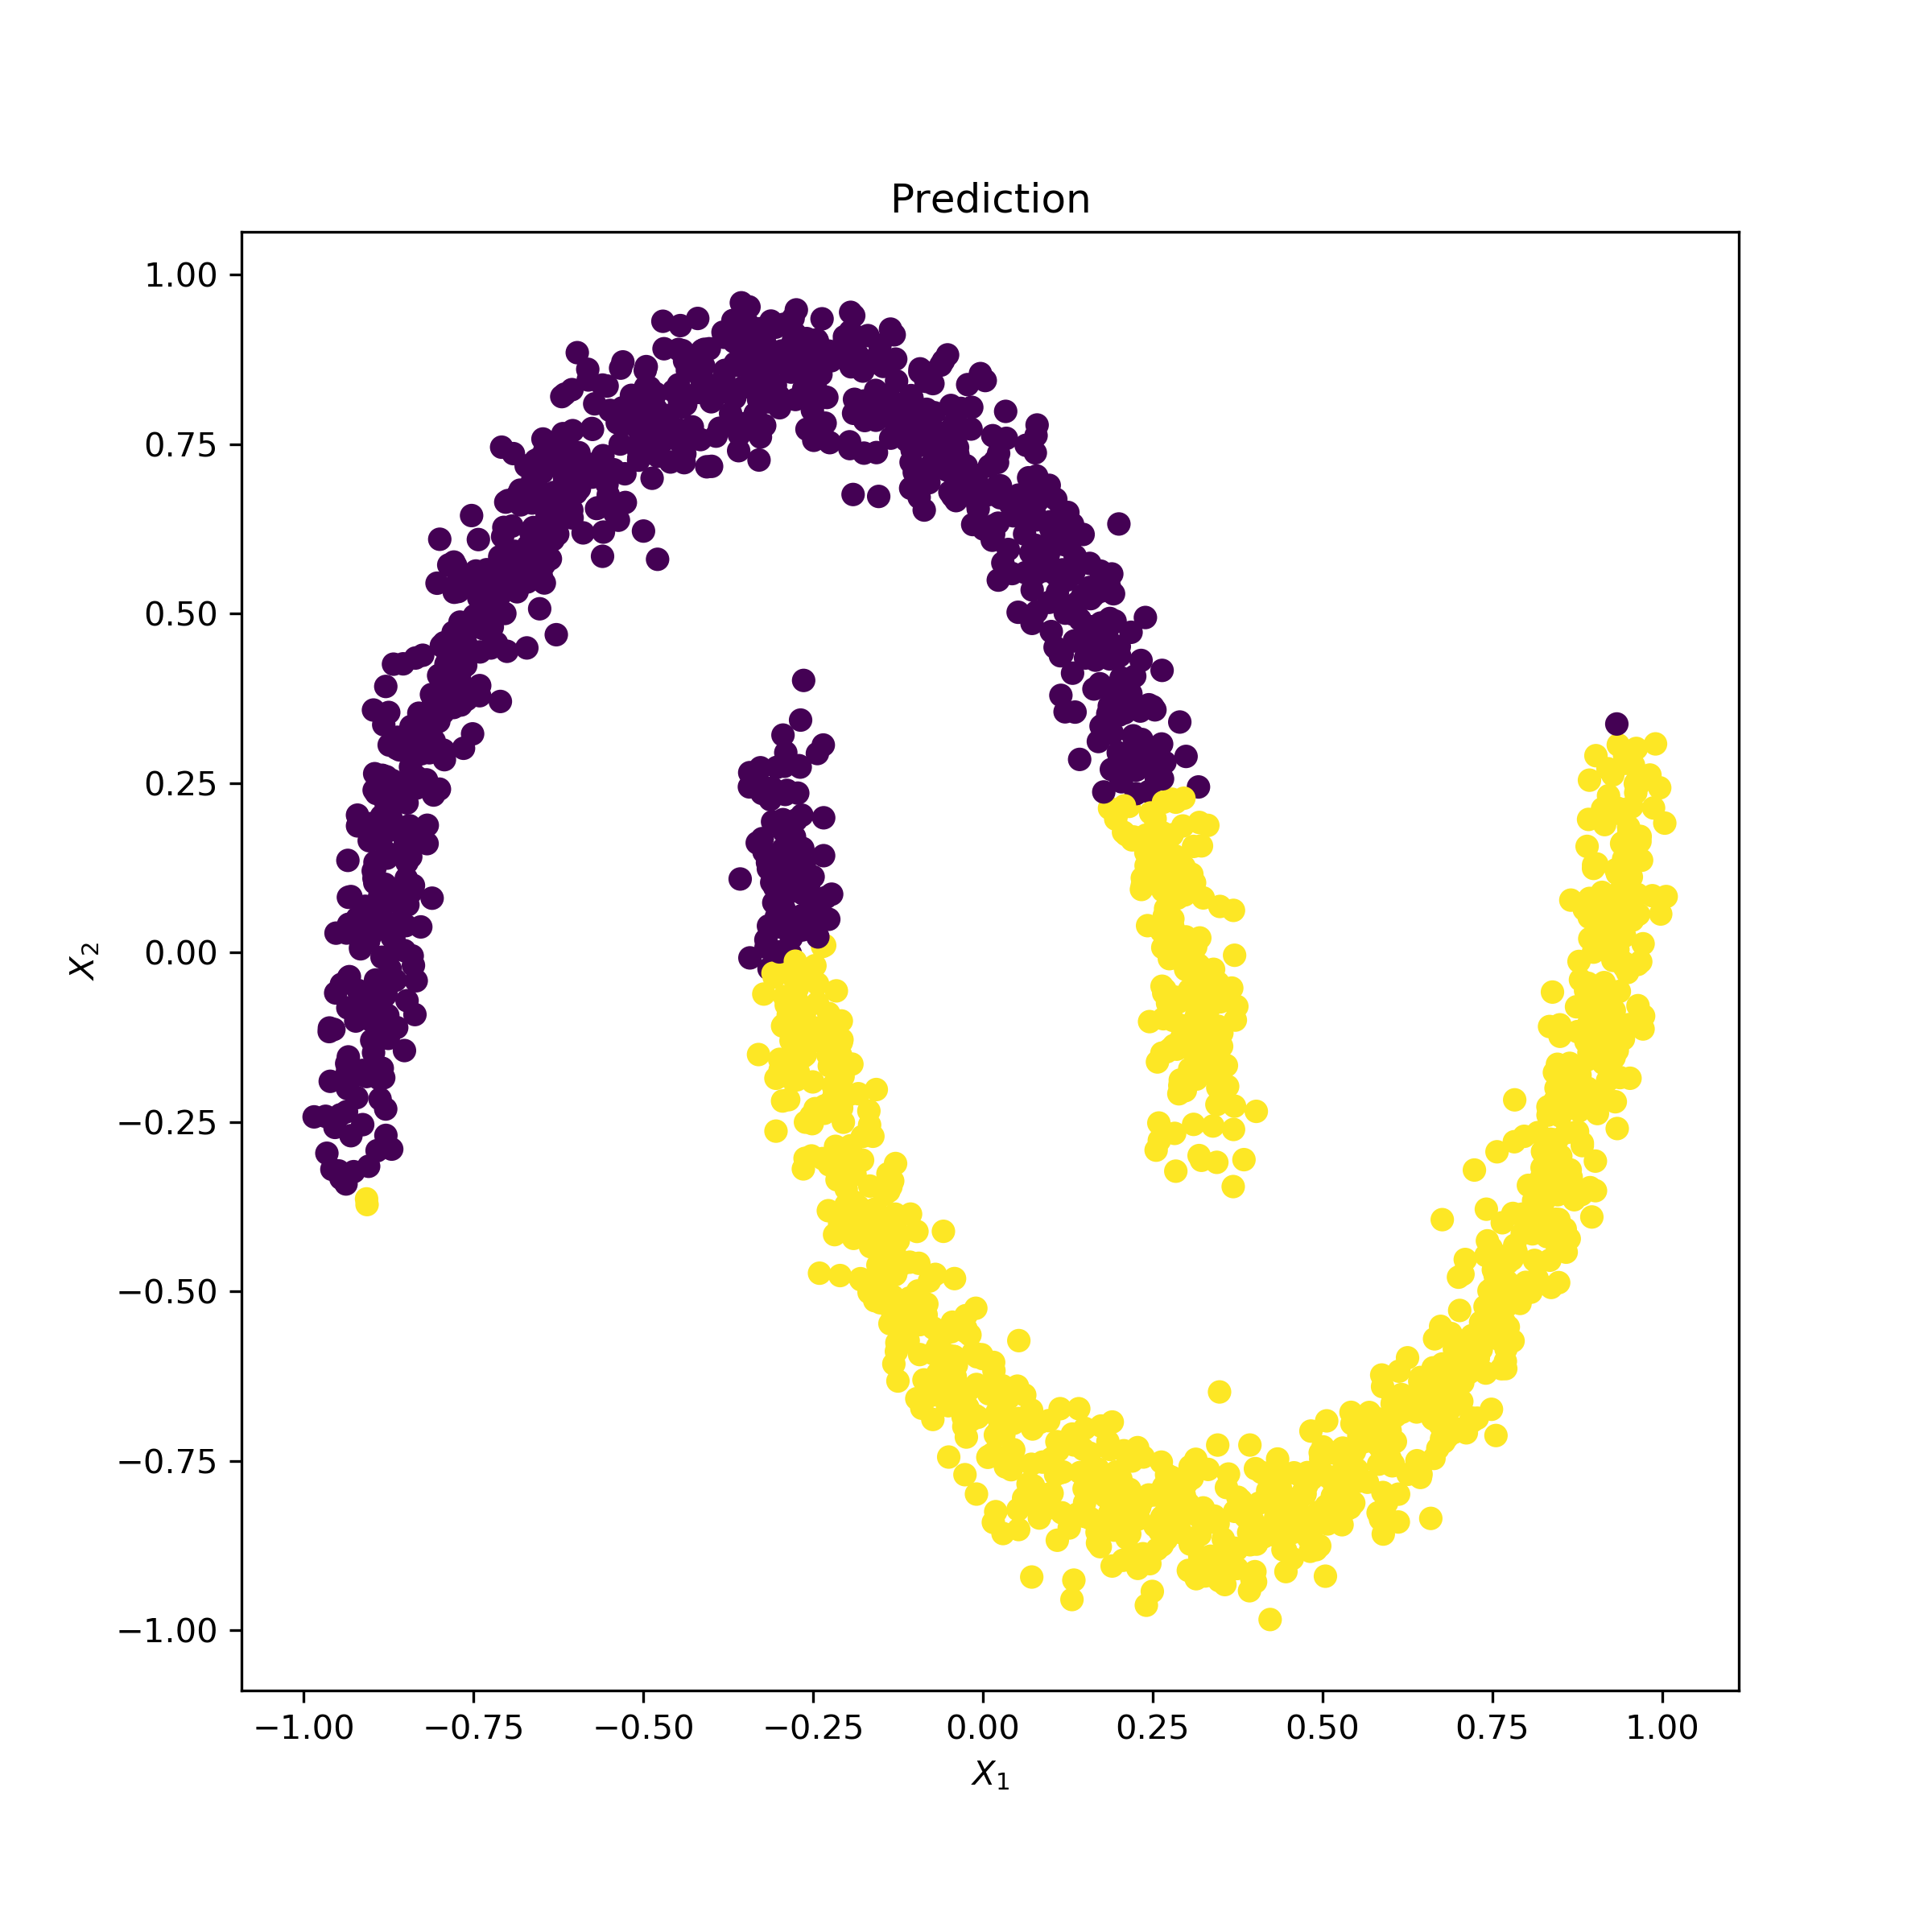
\includegraphics[scale=0.3]{pics/Prediction_i}
	\caption{Classification outcome on test set}
	\label{fig:i_a}
	\end{subfigure}
	\begin{subfigure}{.48\textwidth}
	\centering
	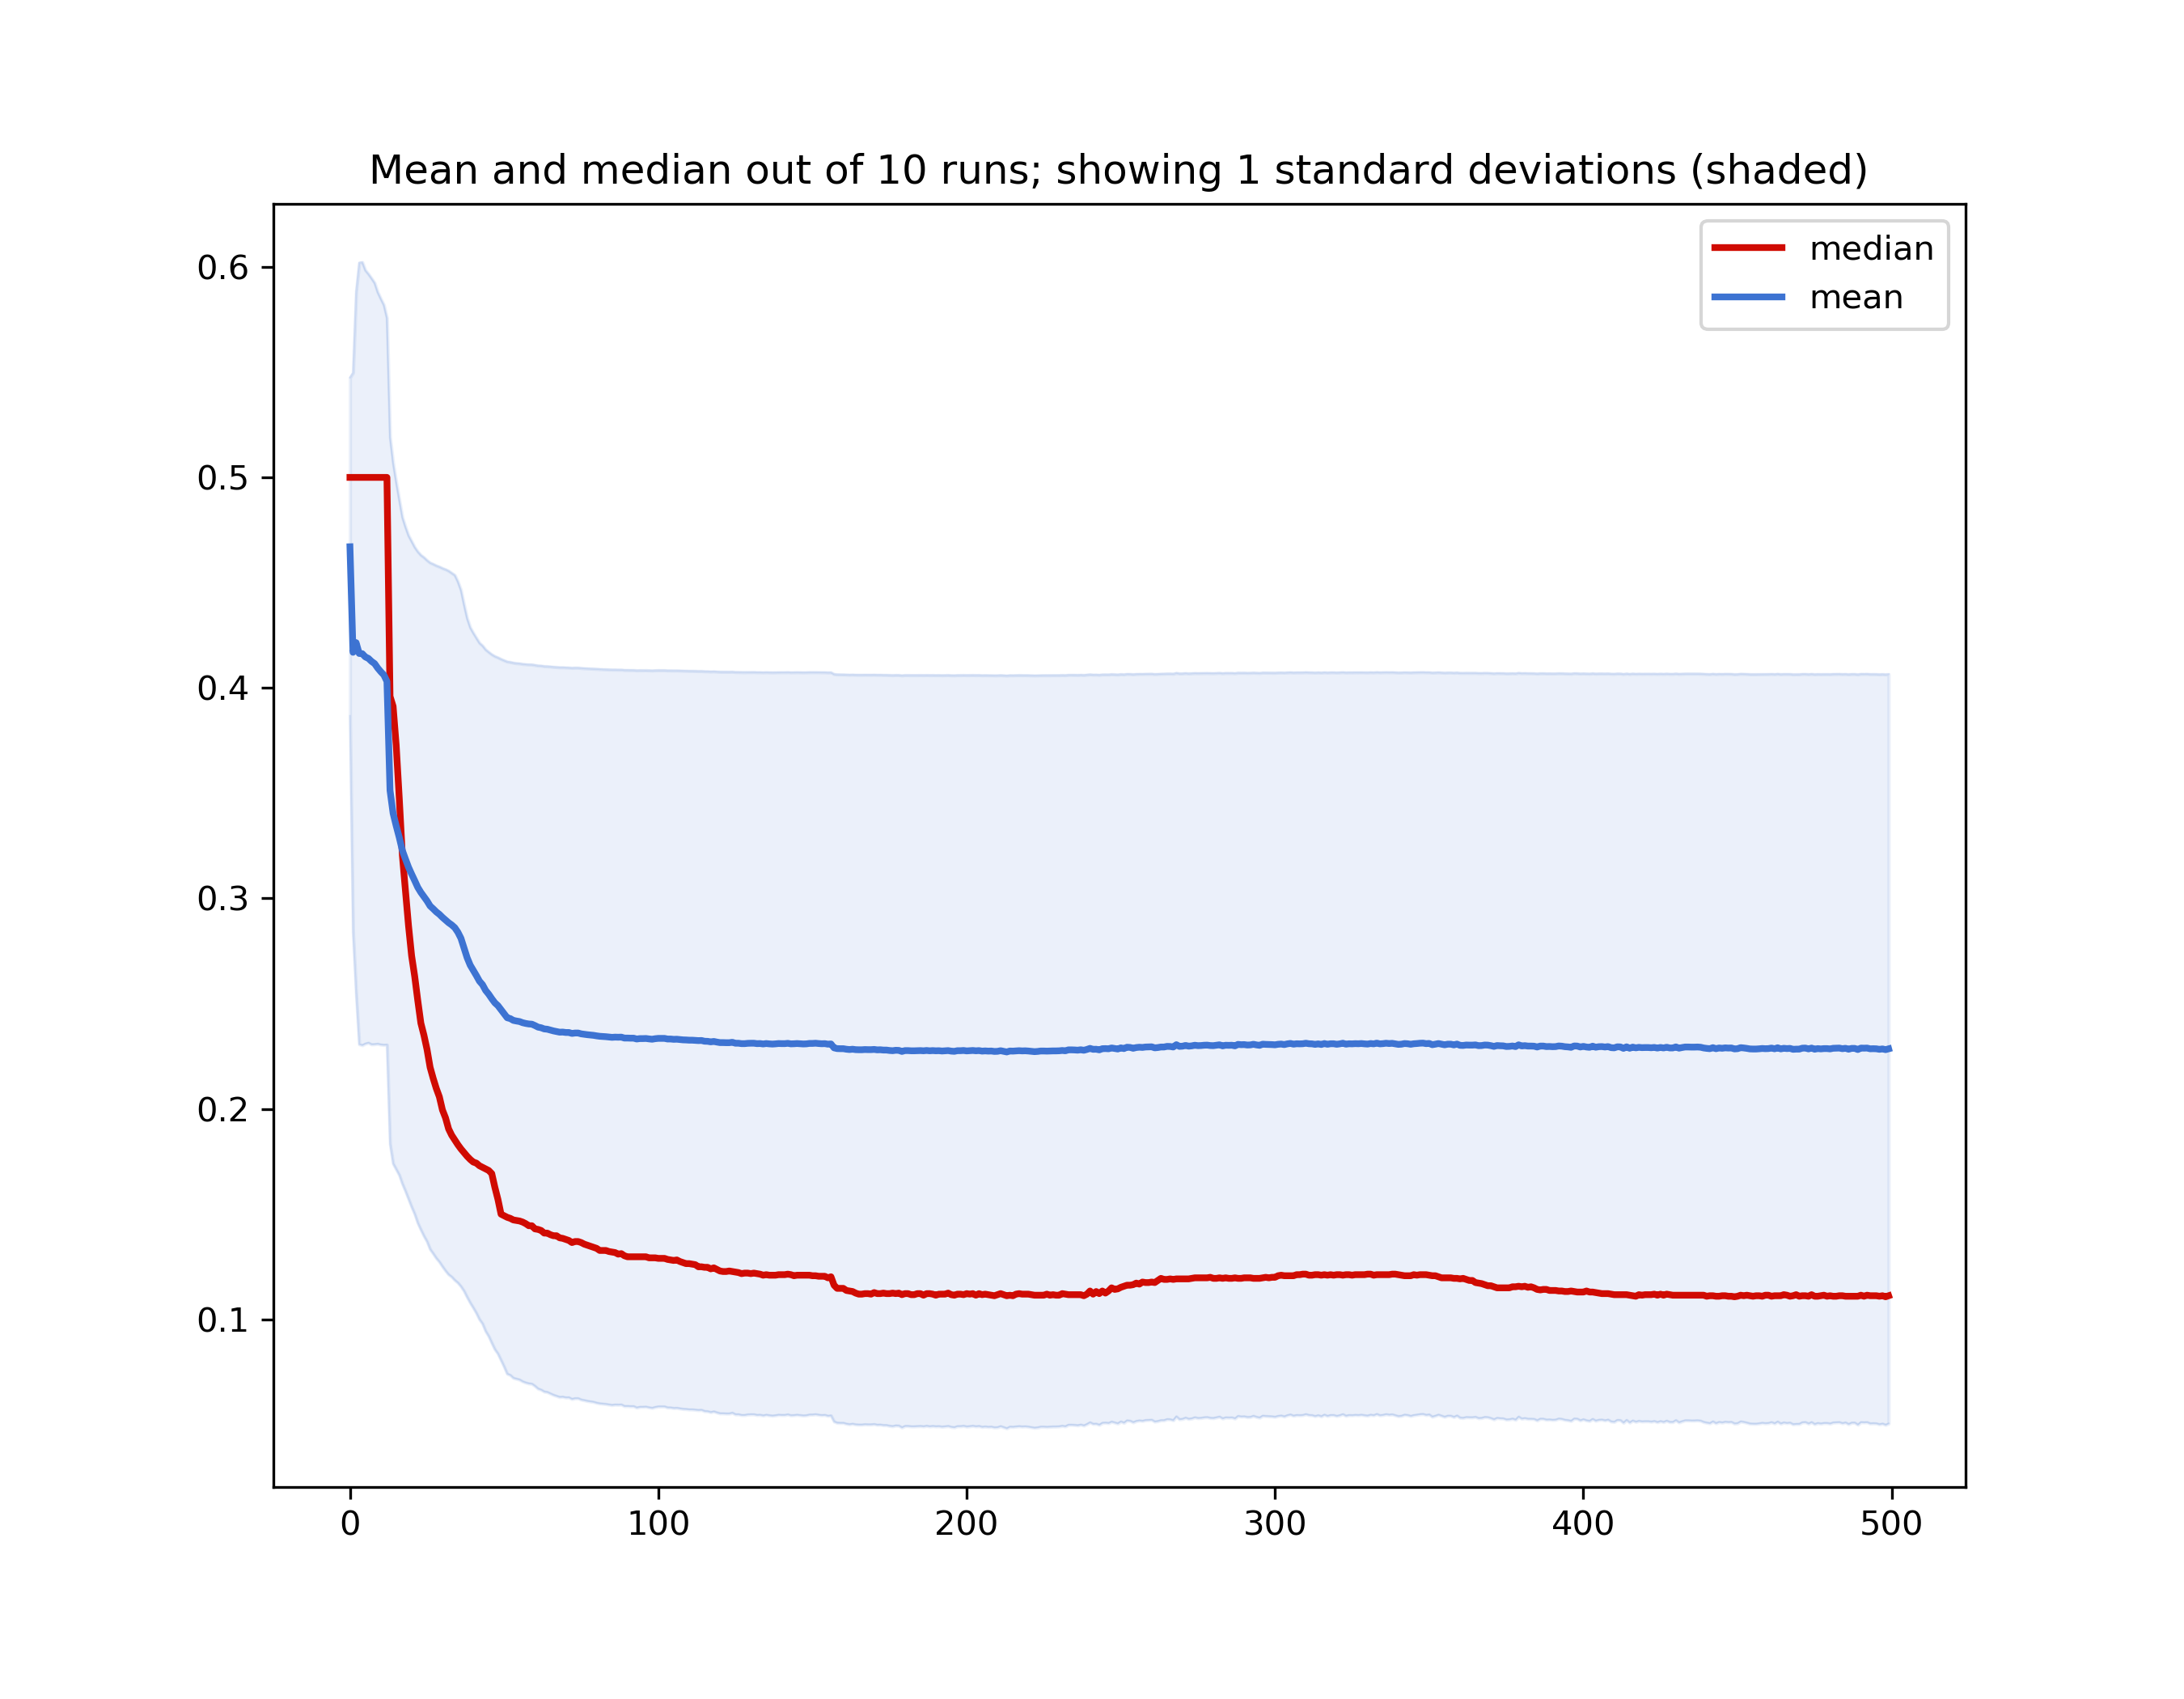
\includegraphics[scale=0.3]{pics/i_ens}
	\caption{Training set error rate: mean and median with standard deviation; composed out of 10 runs.}
	\label{fig:i_b}
	\end{subfigure}
\caption{Error rate on test set: $\gamma_t = 0.1195$. NN is not able to form sufficient decision boundaries.}
\label{fig:res_i}
\end{figure}
\newline
\textbf{ii):} \texttt{layer\_sizes = [3,3, n\_classes]} \\
\begin{figure}[h!]
\captionsetup[subfigure]{labelformat=empty}
\centering
	\begin{subfigure}{.48\textwidth}
	\centering
	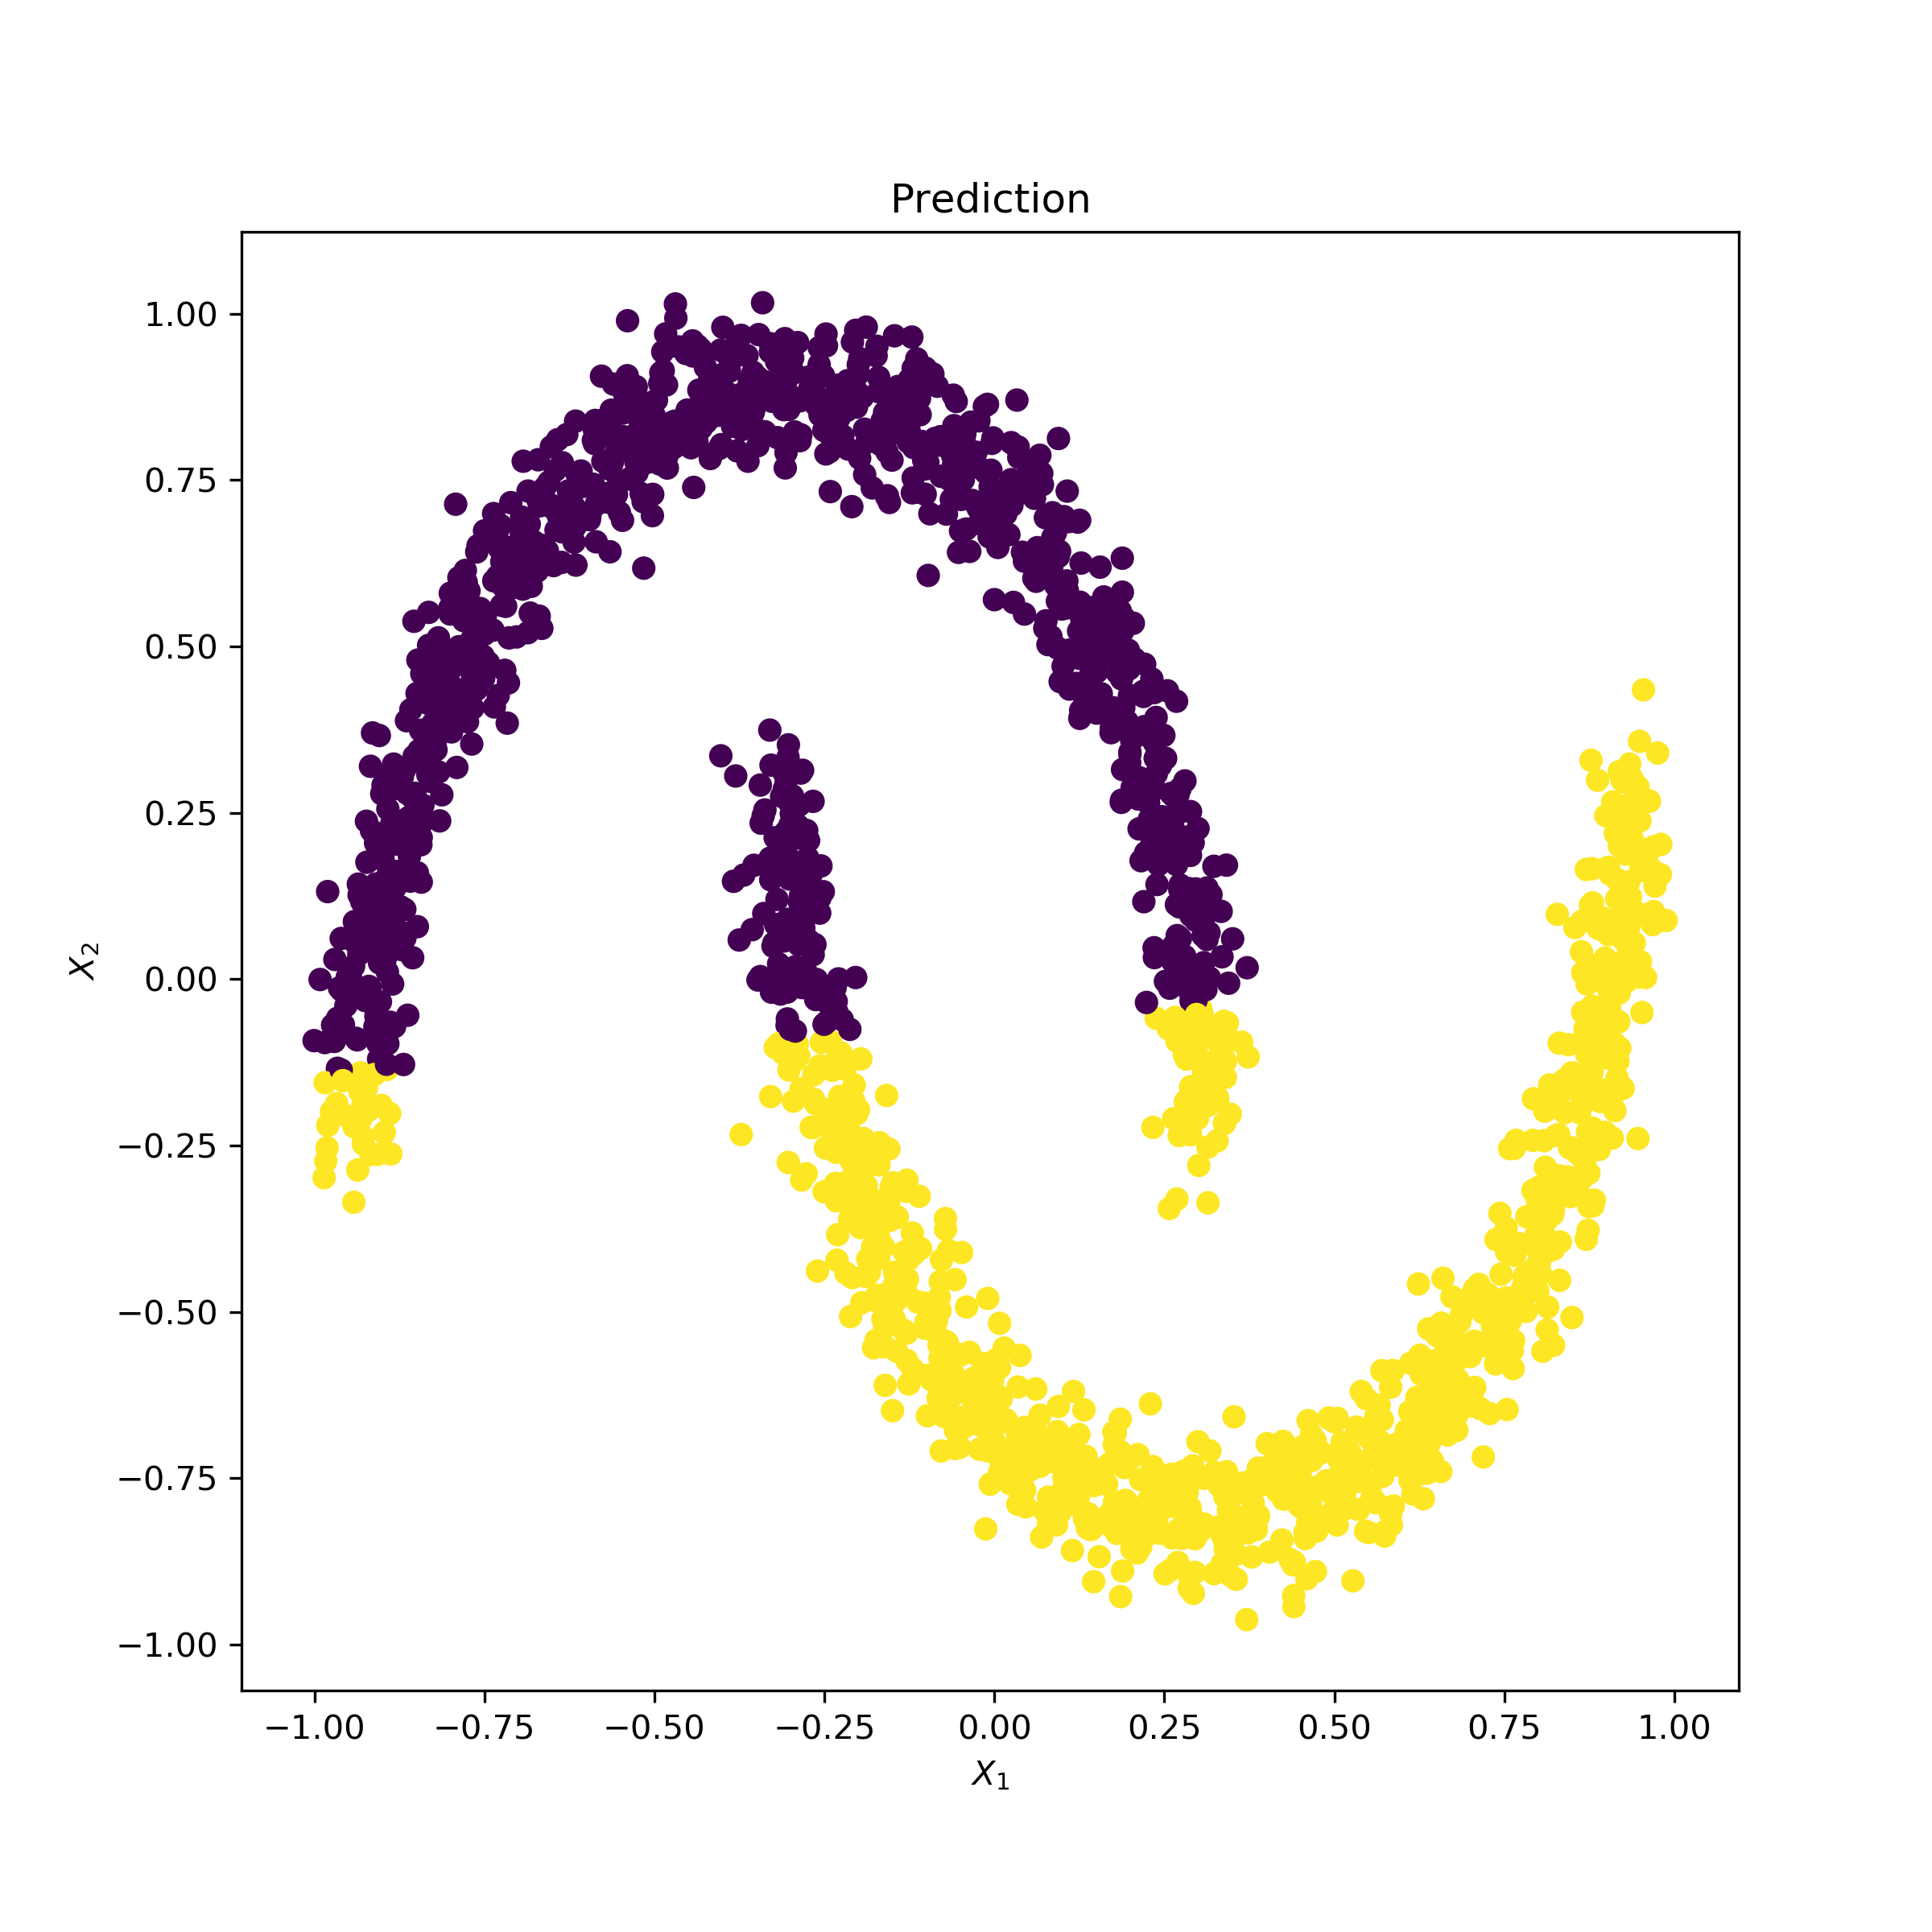
\includegraphics[scale=0.3]{pics/Prediction_ii}
	\caption{Classification outcome on test set}
	\label{fig:ii_a}
	\end{subfigure}
	\begin{subfigure}{.48\textwidth}
	\centering
	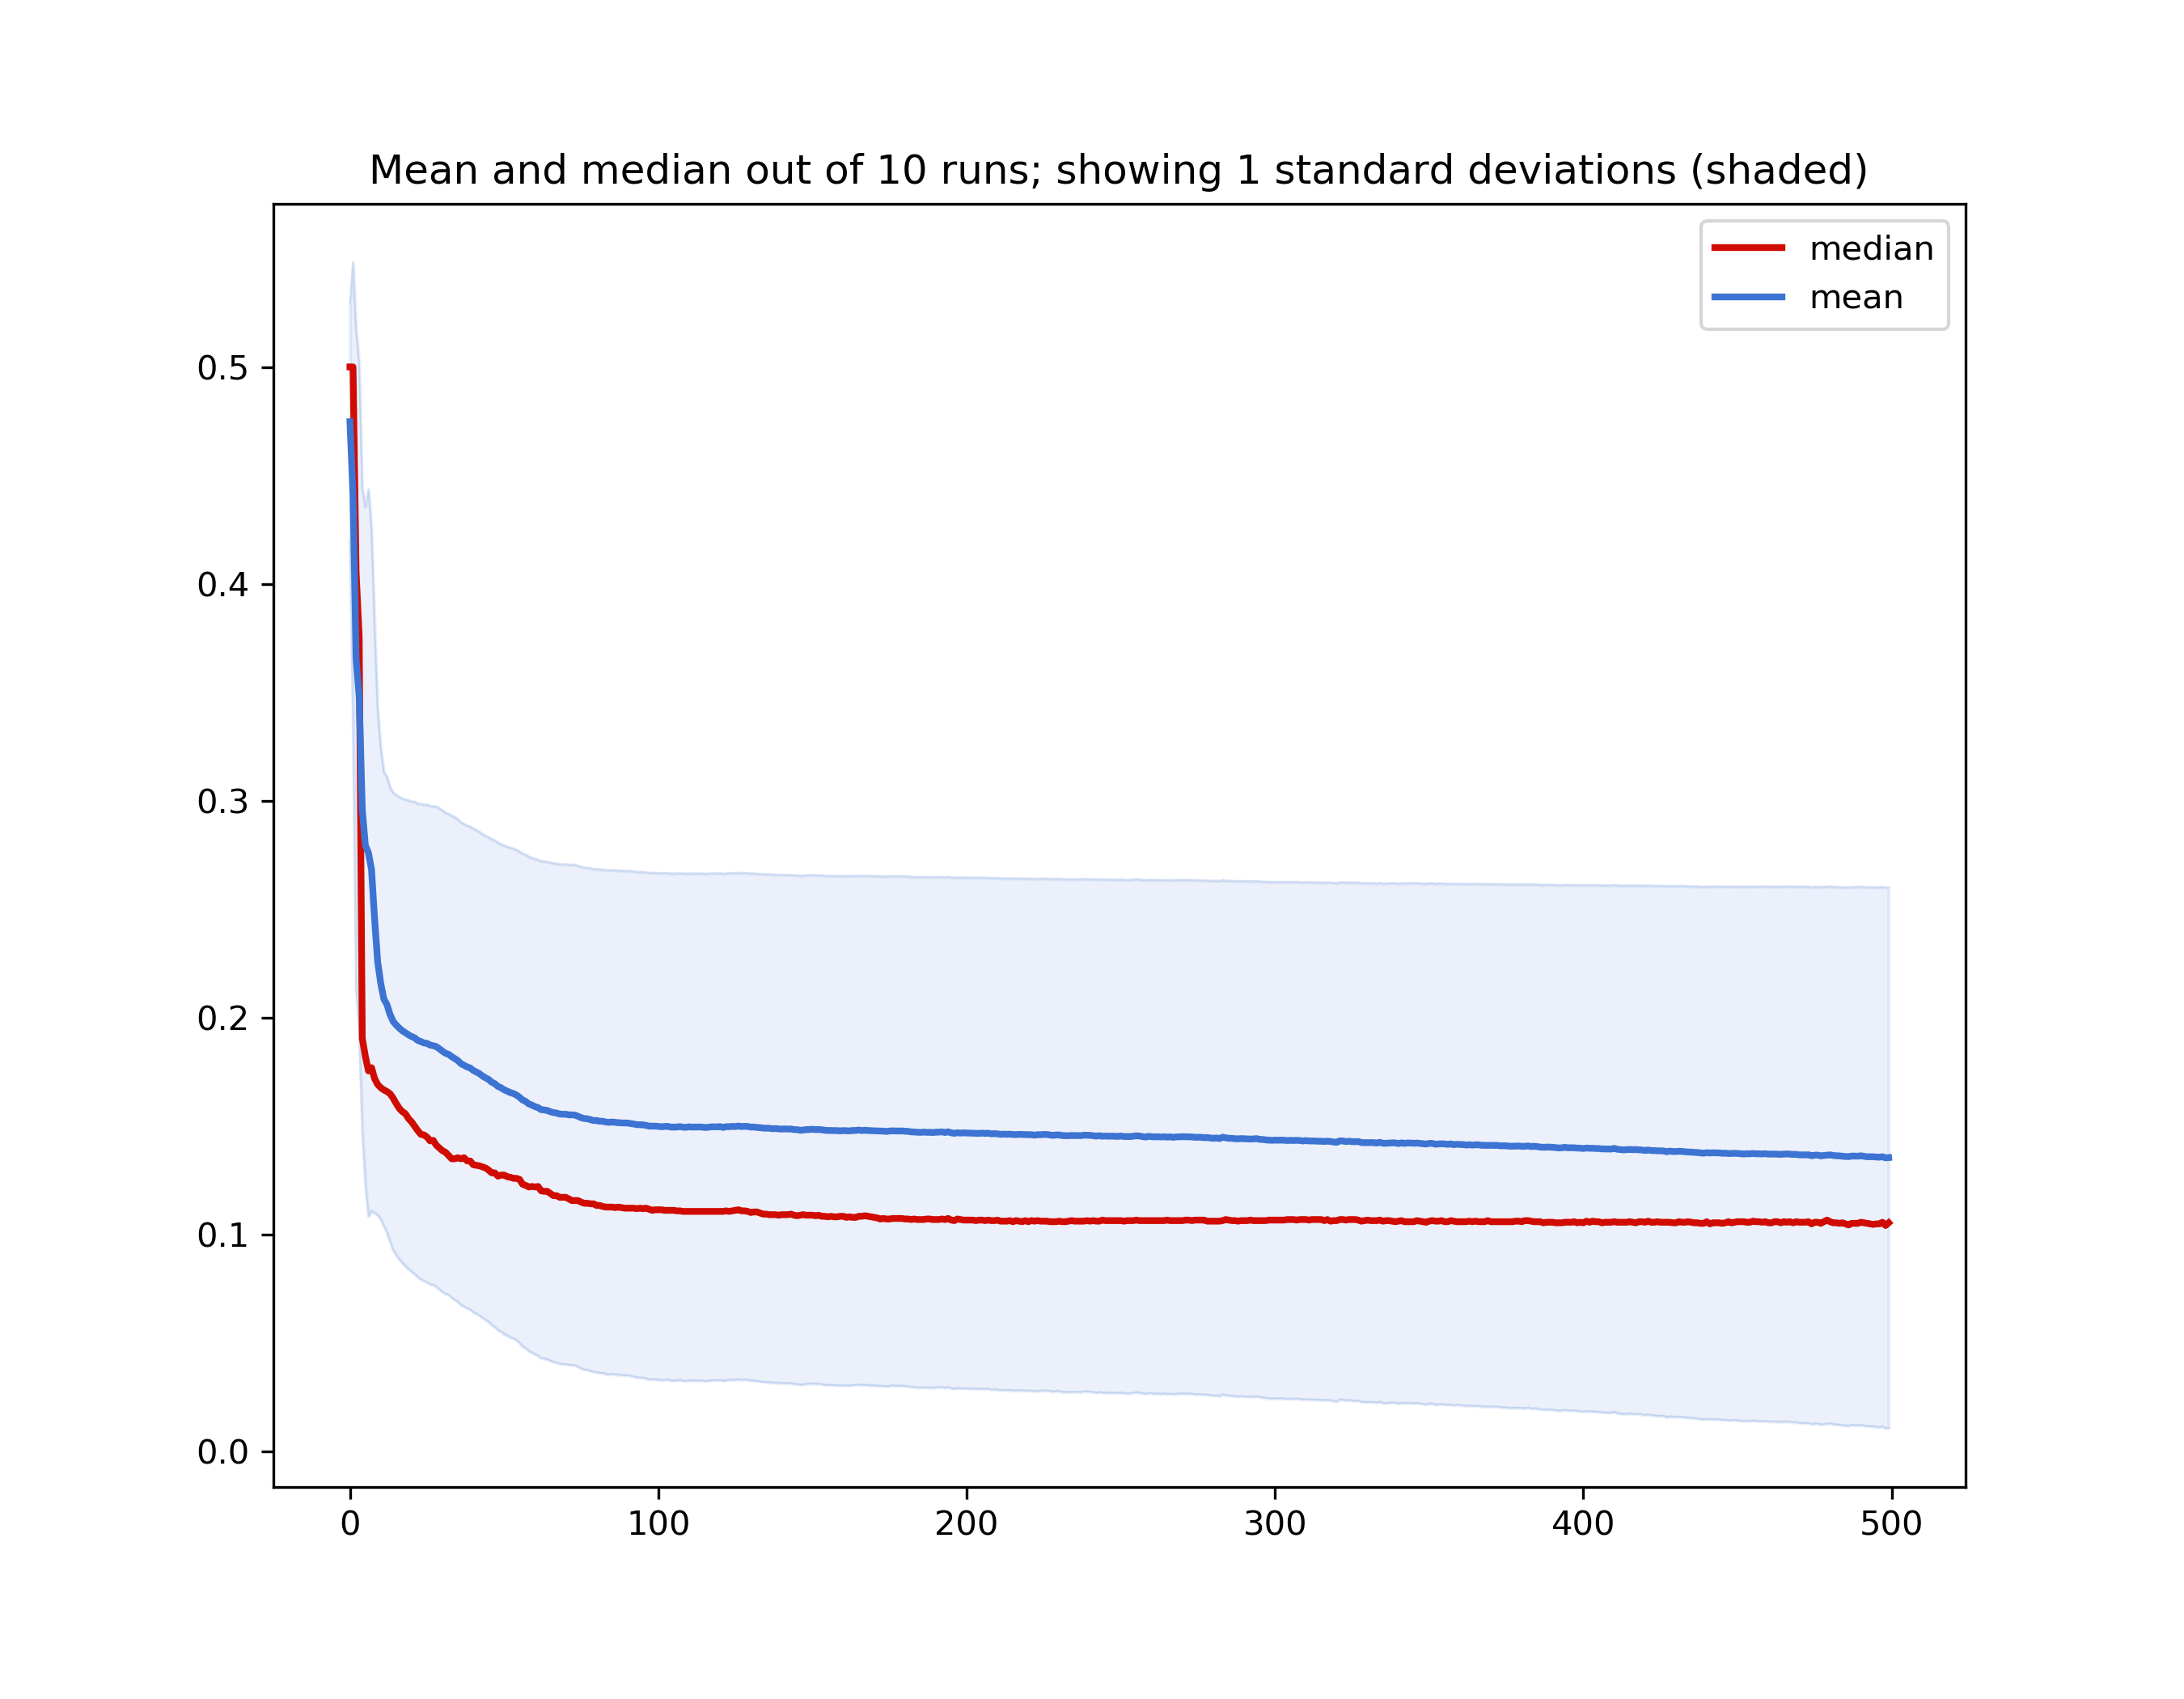
\includegraphics[scale=0.3]{pics/ii_ens}
	\caption{Training set error rate: mean and median with standard deviation; composed out of 10 runs.}
	\label{fig:ii_b}
	\end{subfigure}
\caption{Error rate on test set: $\gamma_t = 0.104$. NN is still not able to form sufficient decision boundaries.}
\label{fig:res_ii}
\end{figure}
\newpage
\enlargethispage{10\baselineskip}
\noindent \textbf{iii):} \texttt{layer\_sizes = [5,5, n\_classes]} \\
\begin{figure}[htbp]
\captionsetup[subfigure]{labelformat=empty}
\centering
	\begin{subfigure}{.48\textwidth}
	\centering
	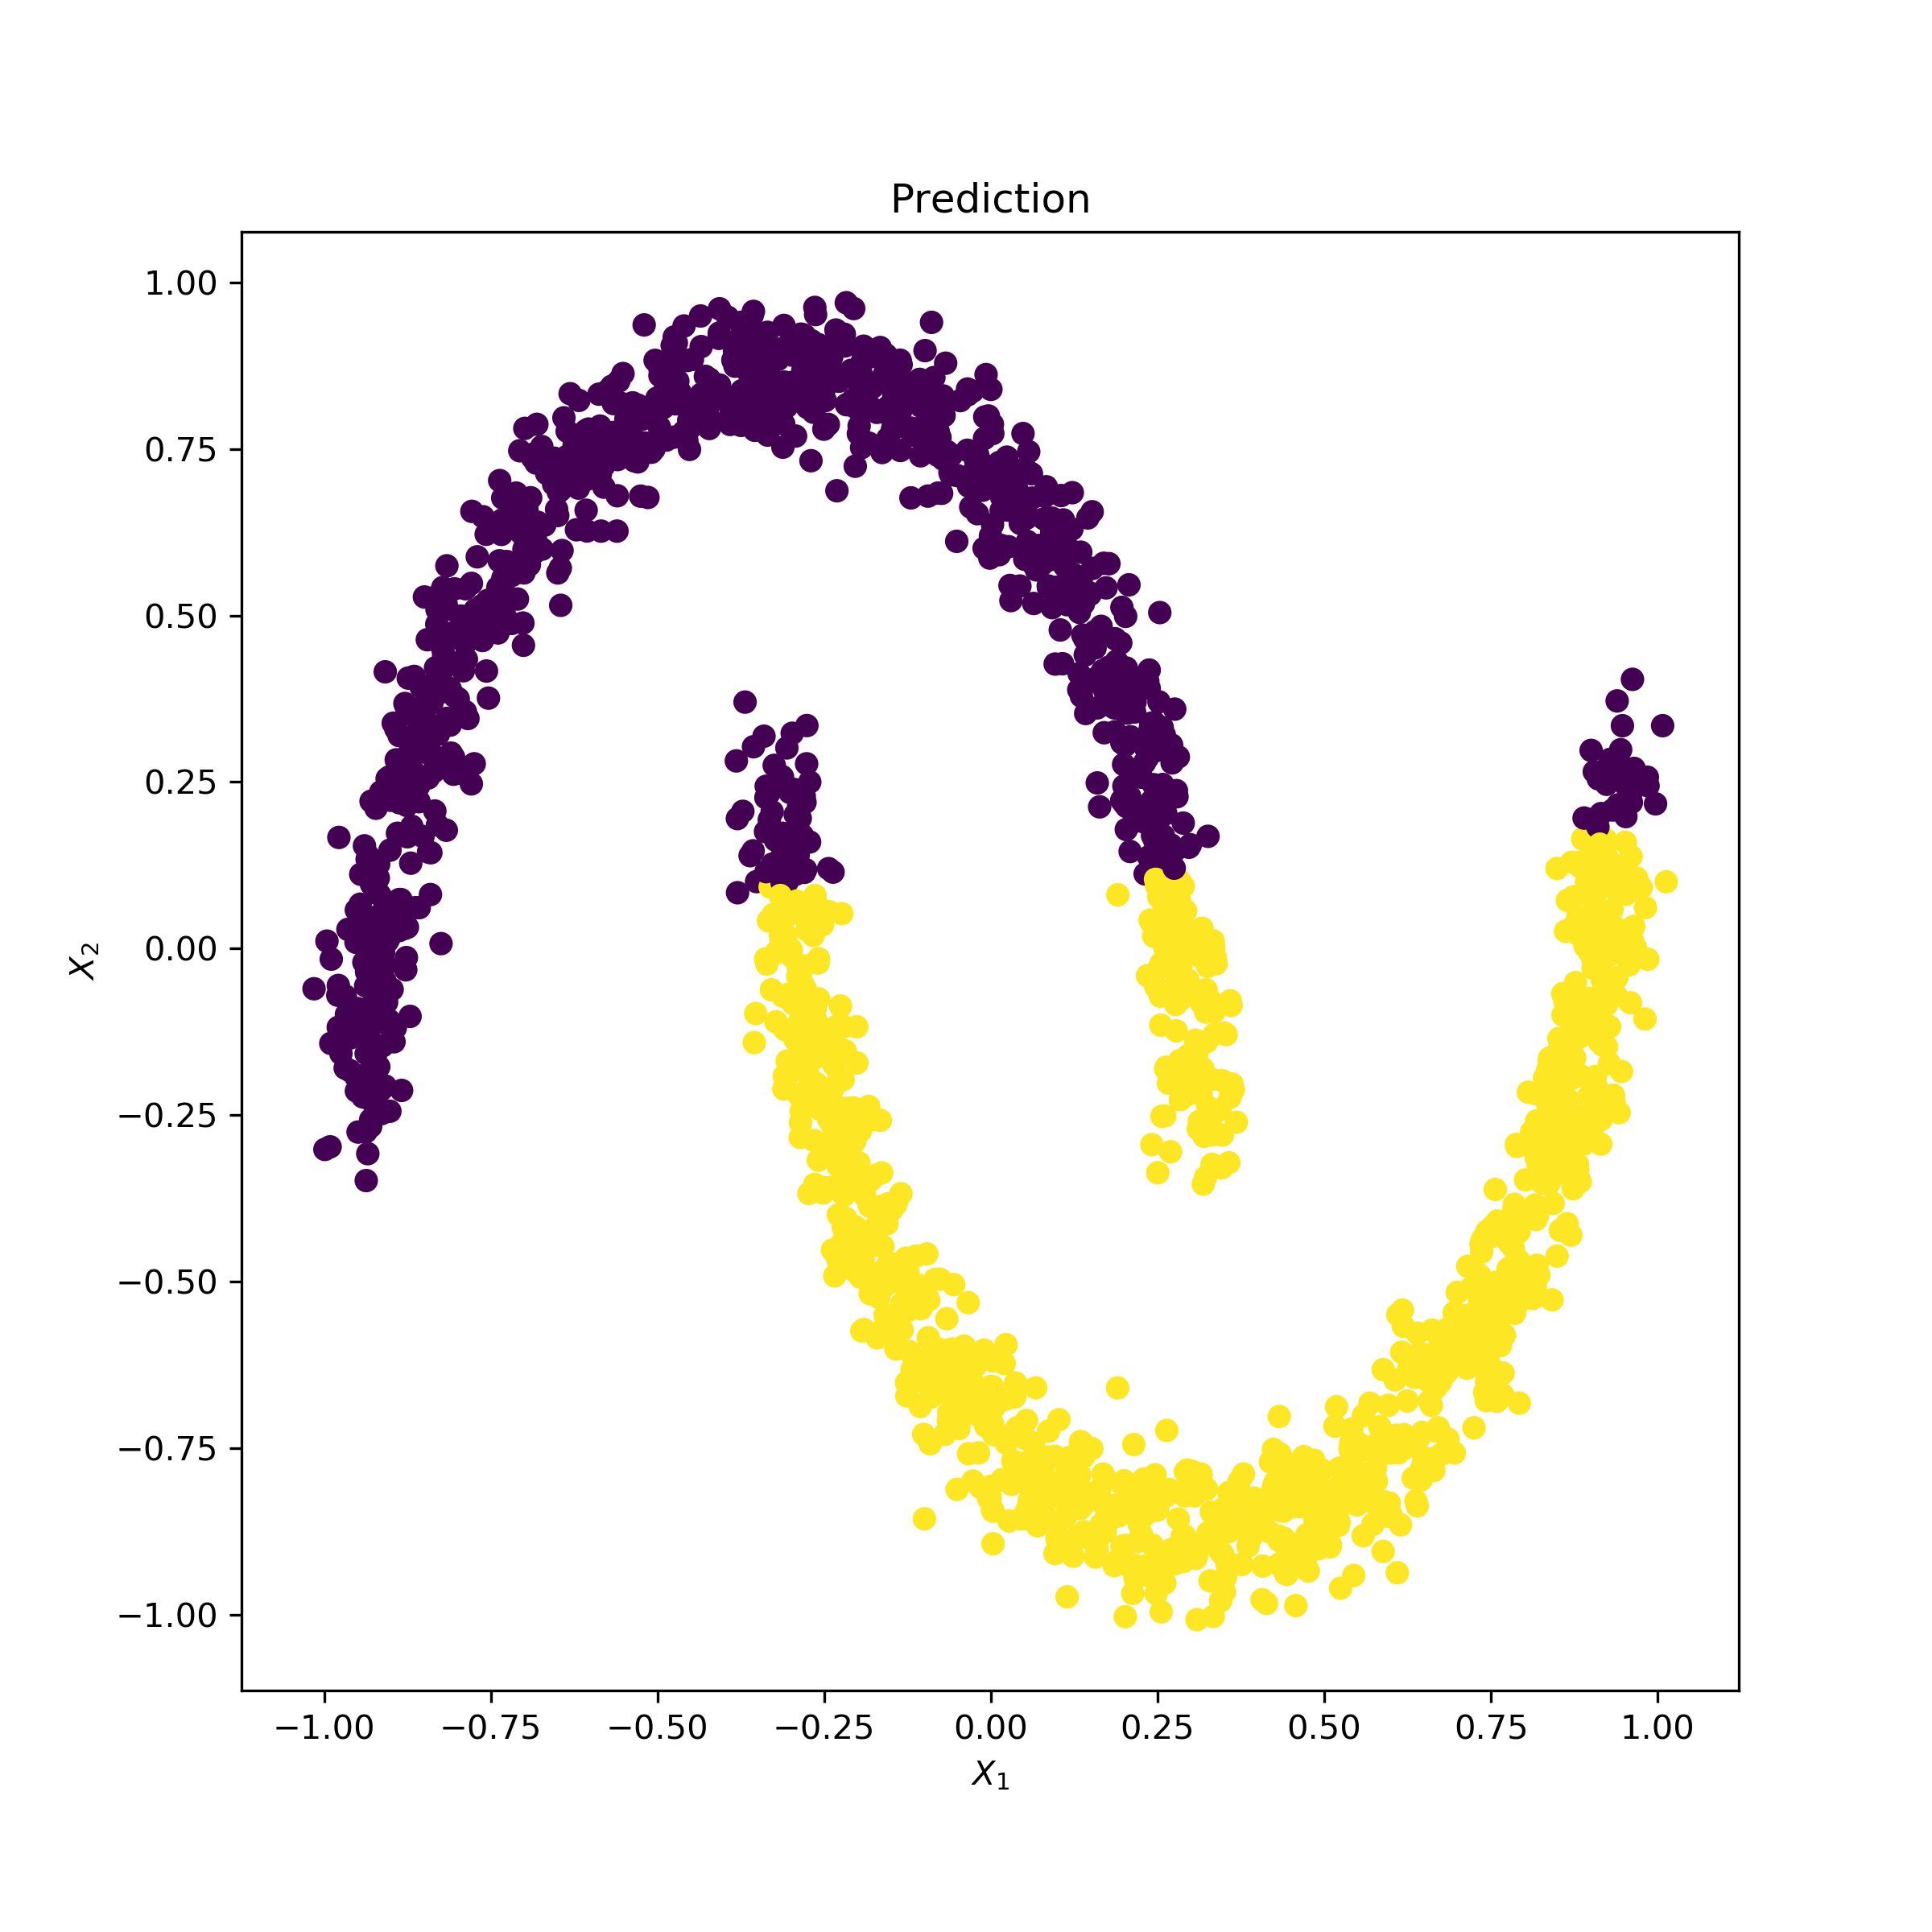
\includegraphics[scale=0.30]{pics/Prediction_iii}
	\caption{Classification outcome on test set}
	\label{fig:iii_a}
	\end{subfigure}
	\begin{subfigure}{.48\textwidth}
	\centering
	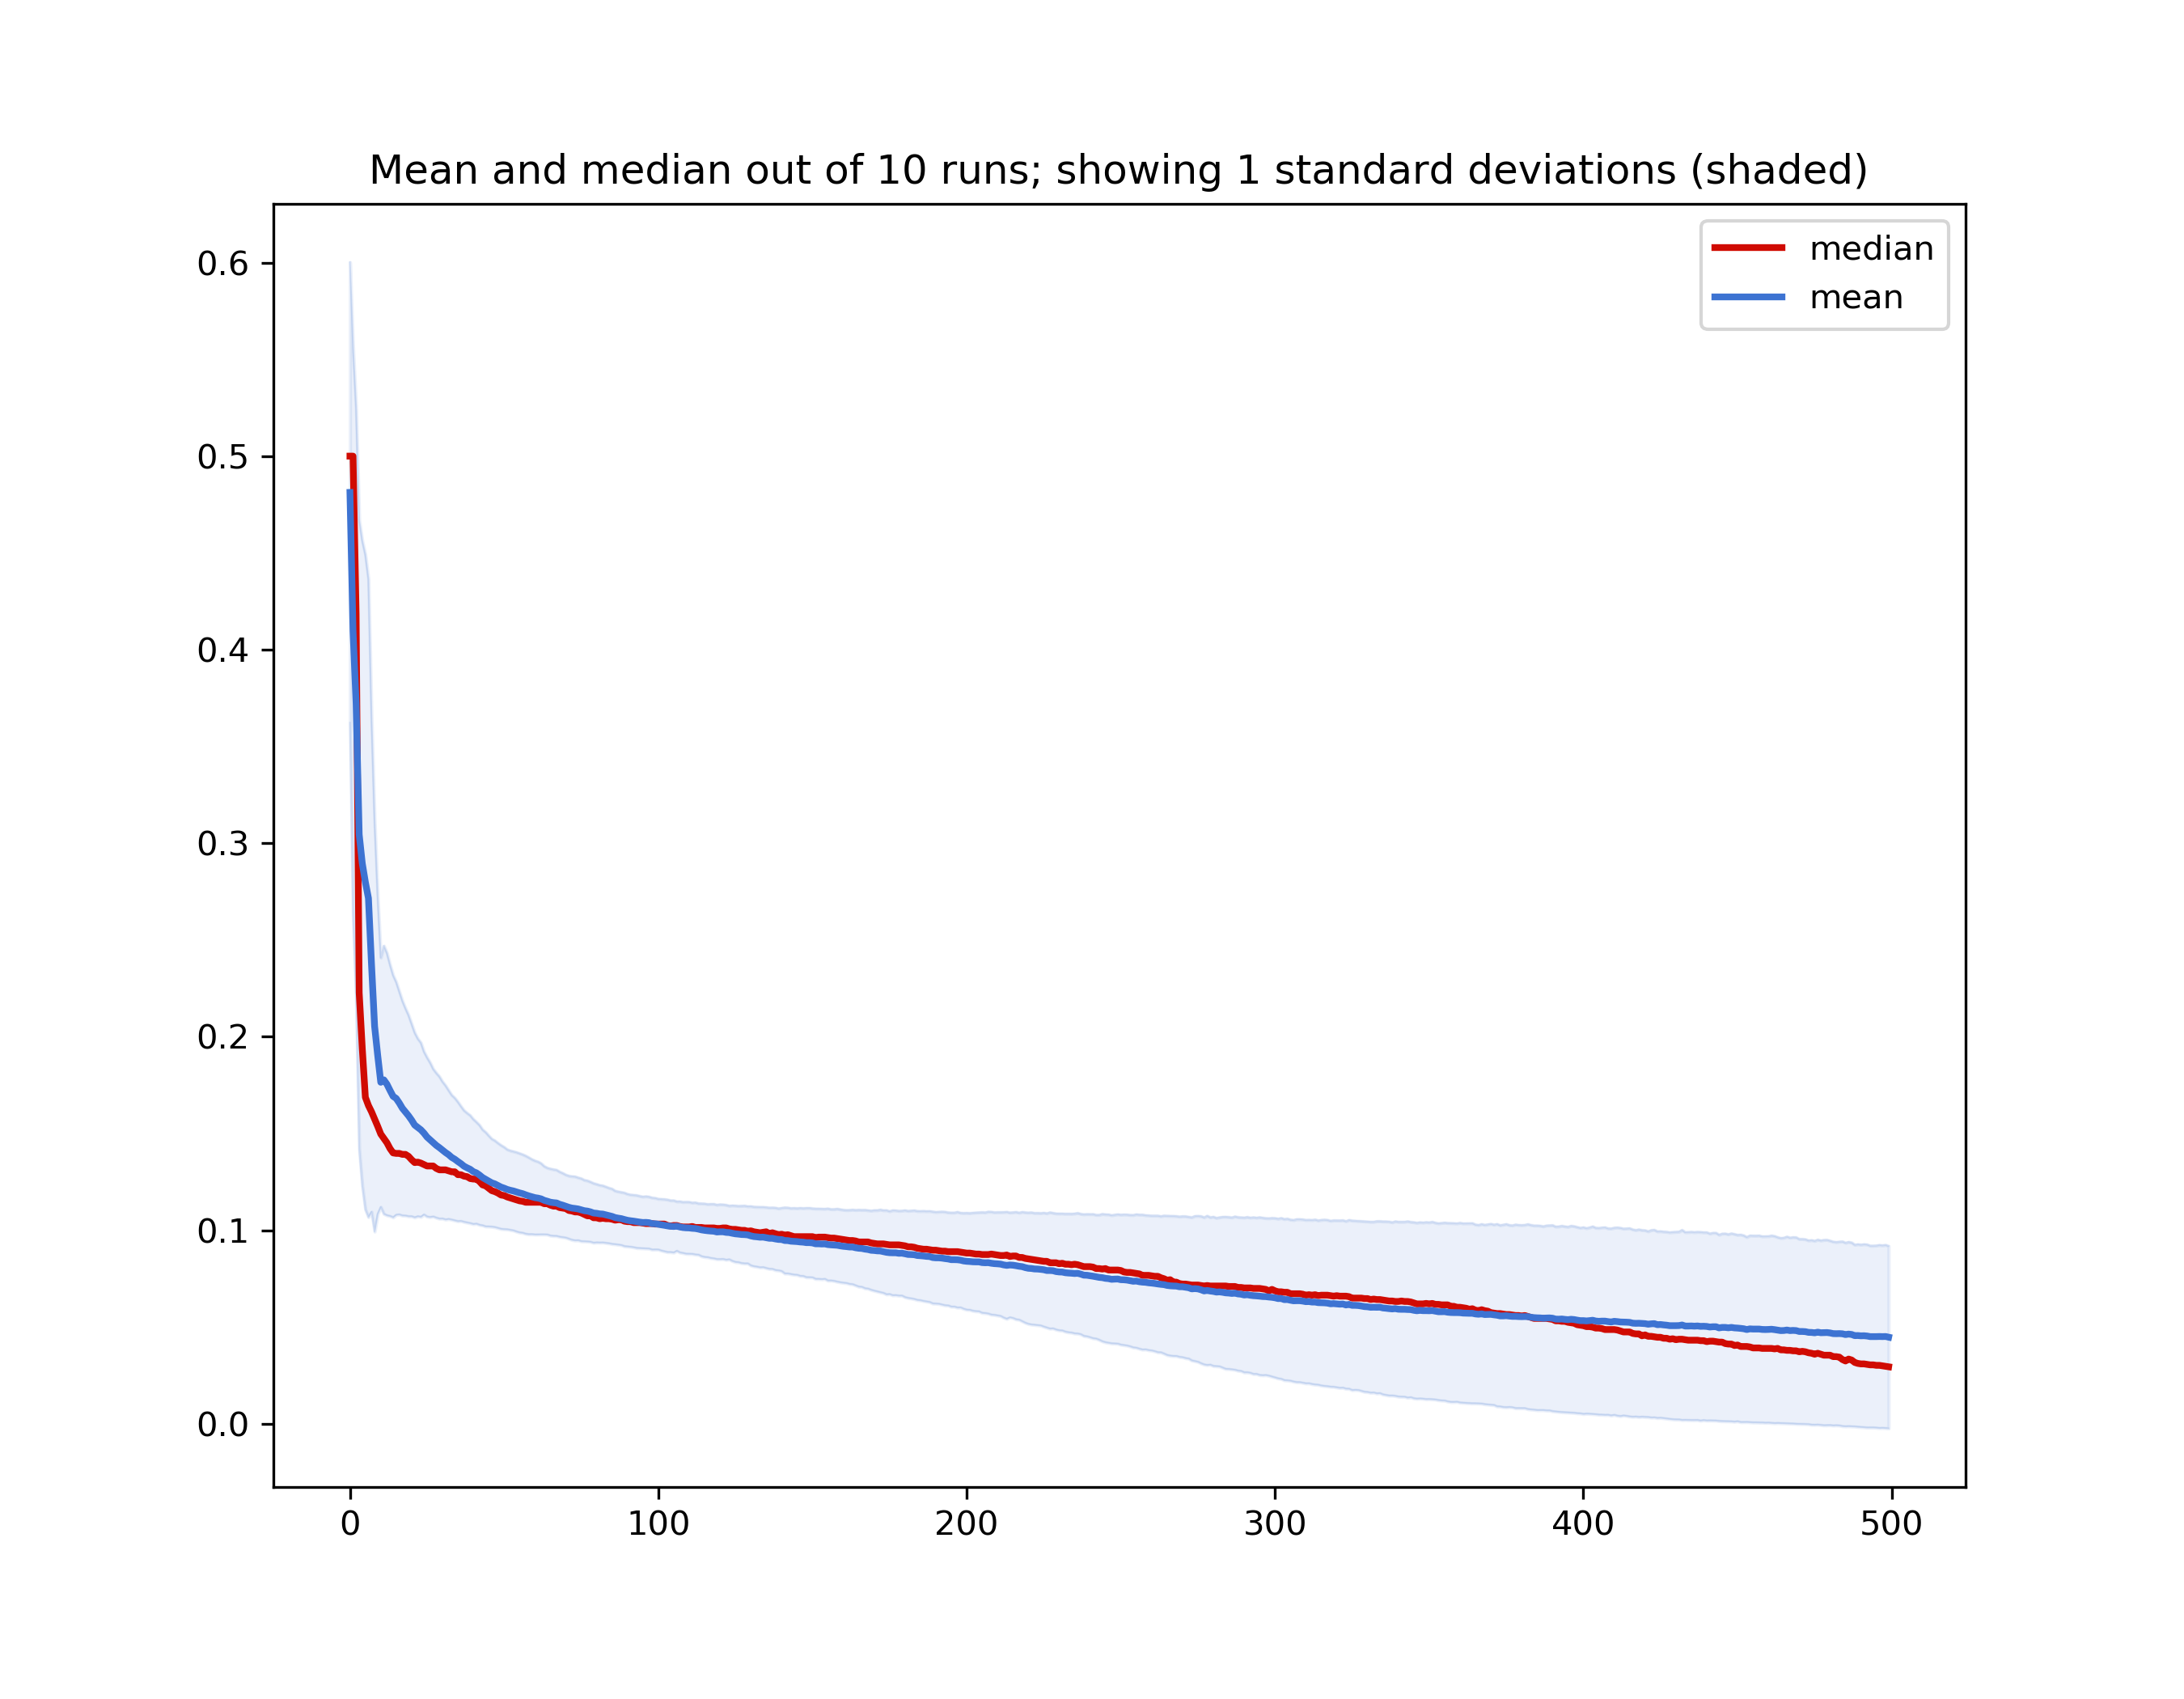
\includegraphics[scale=0.30]{pics/iii_ens}
	\caption{Training set error rate: mean and median with standard deviation; composed out of 10 runs.}
	\label{fig:iii_b}
	\end{subfigure}
\caption{Error rate on test set: $\gamma_t = 0.0985$. NN begins to form sufficient decision boundaries.}
\label{fig:res_iii}
\end{figure}
\newline
\noindent \textbf{iv):} \texttt{layer\_sizes = [30,30, n\_classes]} \\
\begin{figure}[h!]
\captionsetup[subfigure]{labelformat=empty}
\centering
	\begin{subfigure}{.48\textwidth}
	\centering
	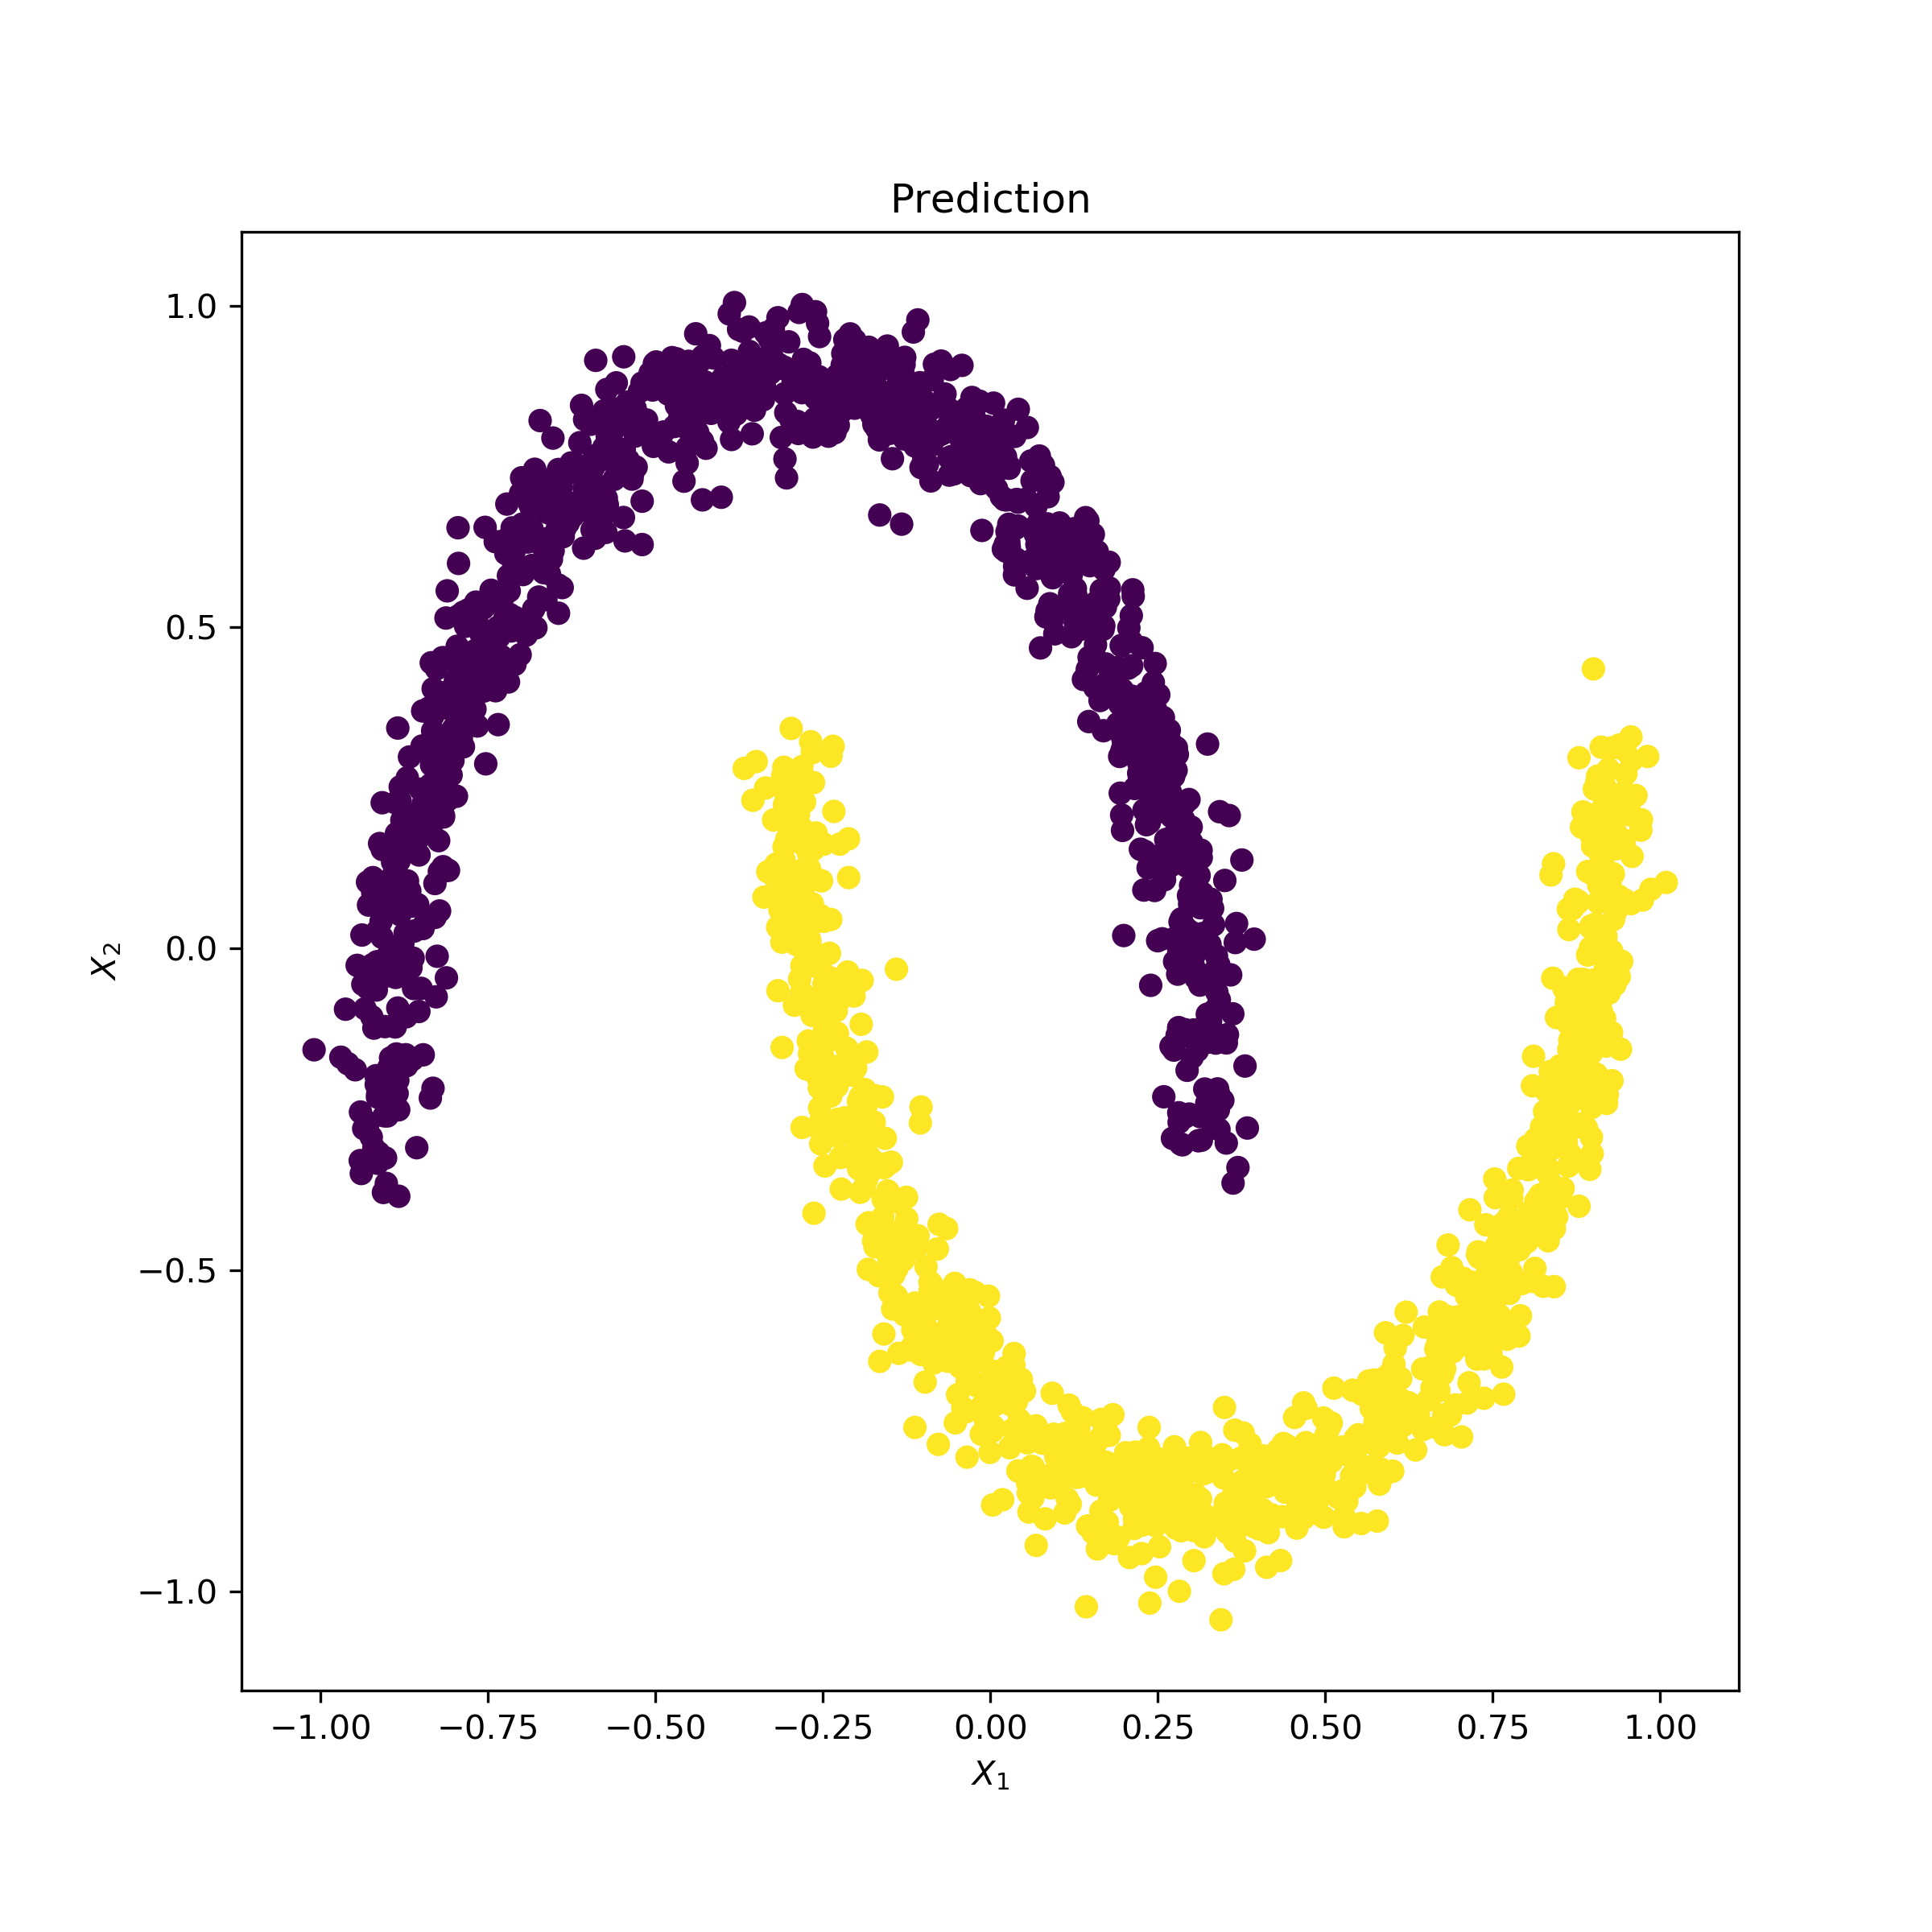
\includegraphics[scale=0.30]{pics/Prediction_4}
	\caption{Classification outcome on test set}
	\label{fig:iv_a}
	\end{subfigure}
	\begin{subfigure}{.48\textwidth}
	\centering
	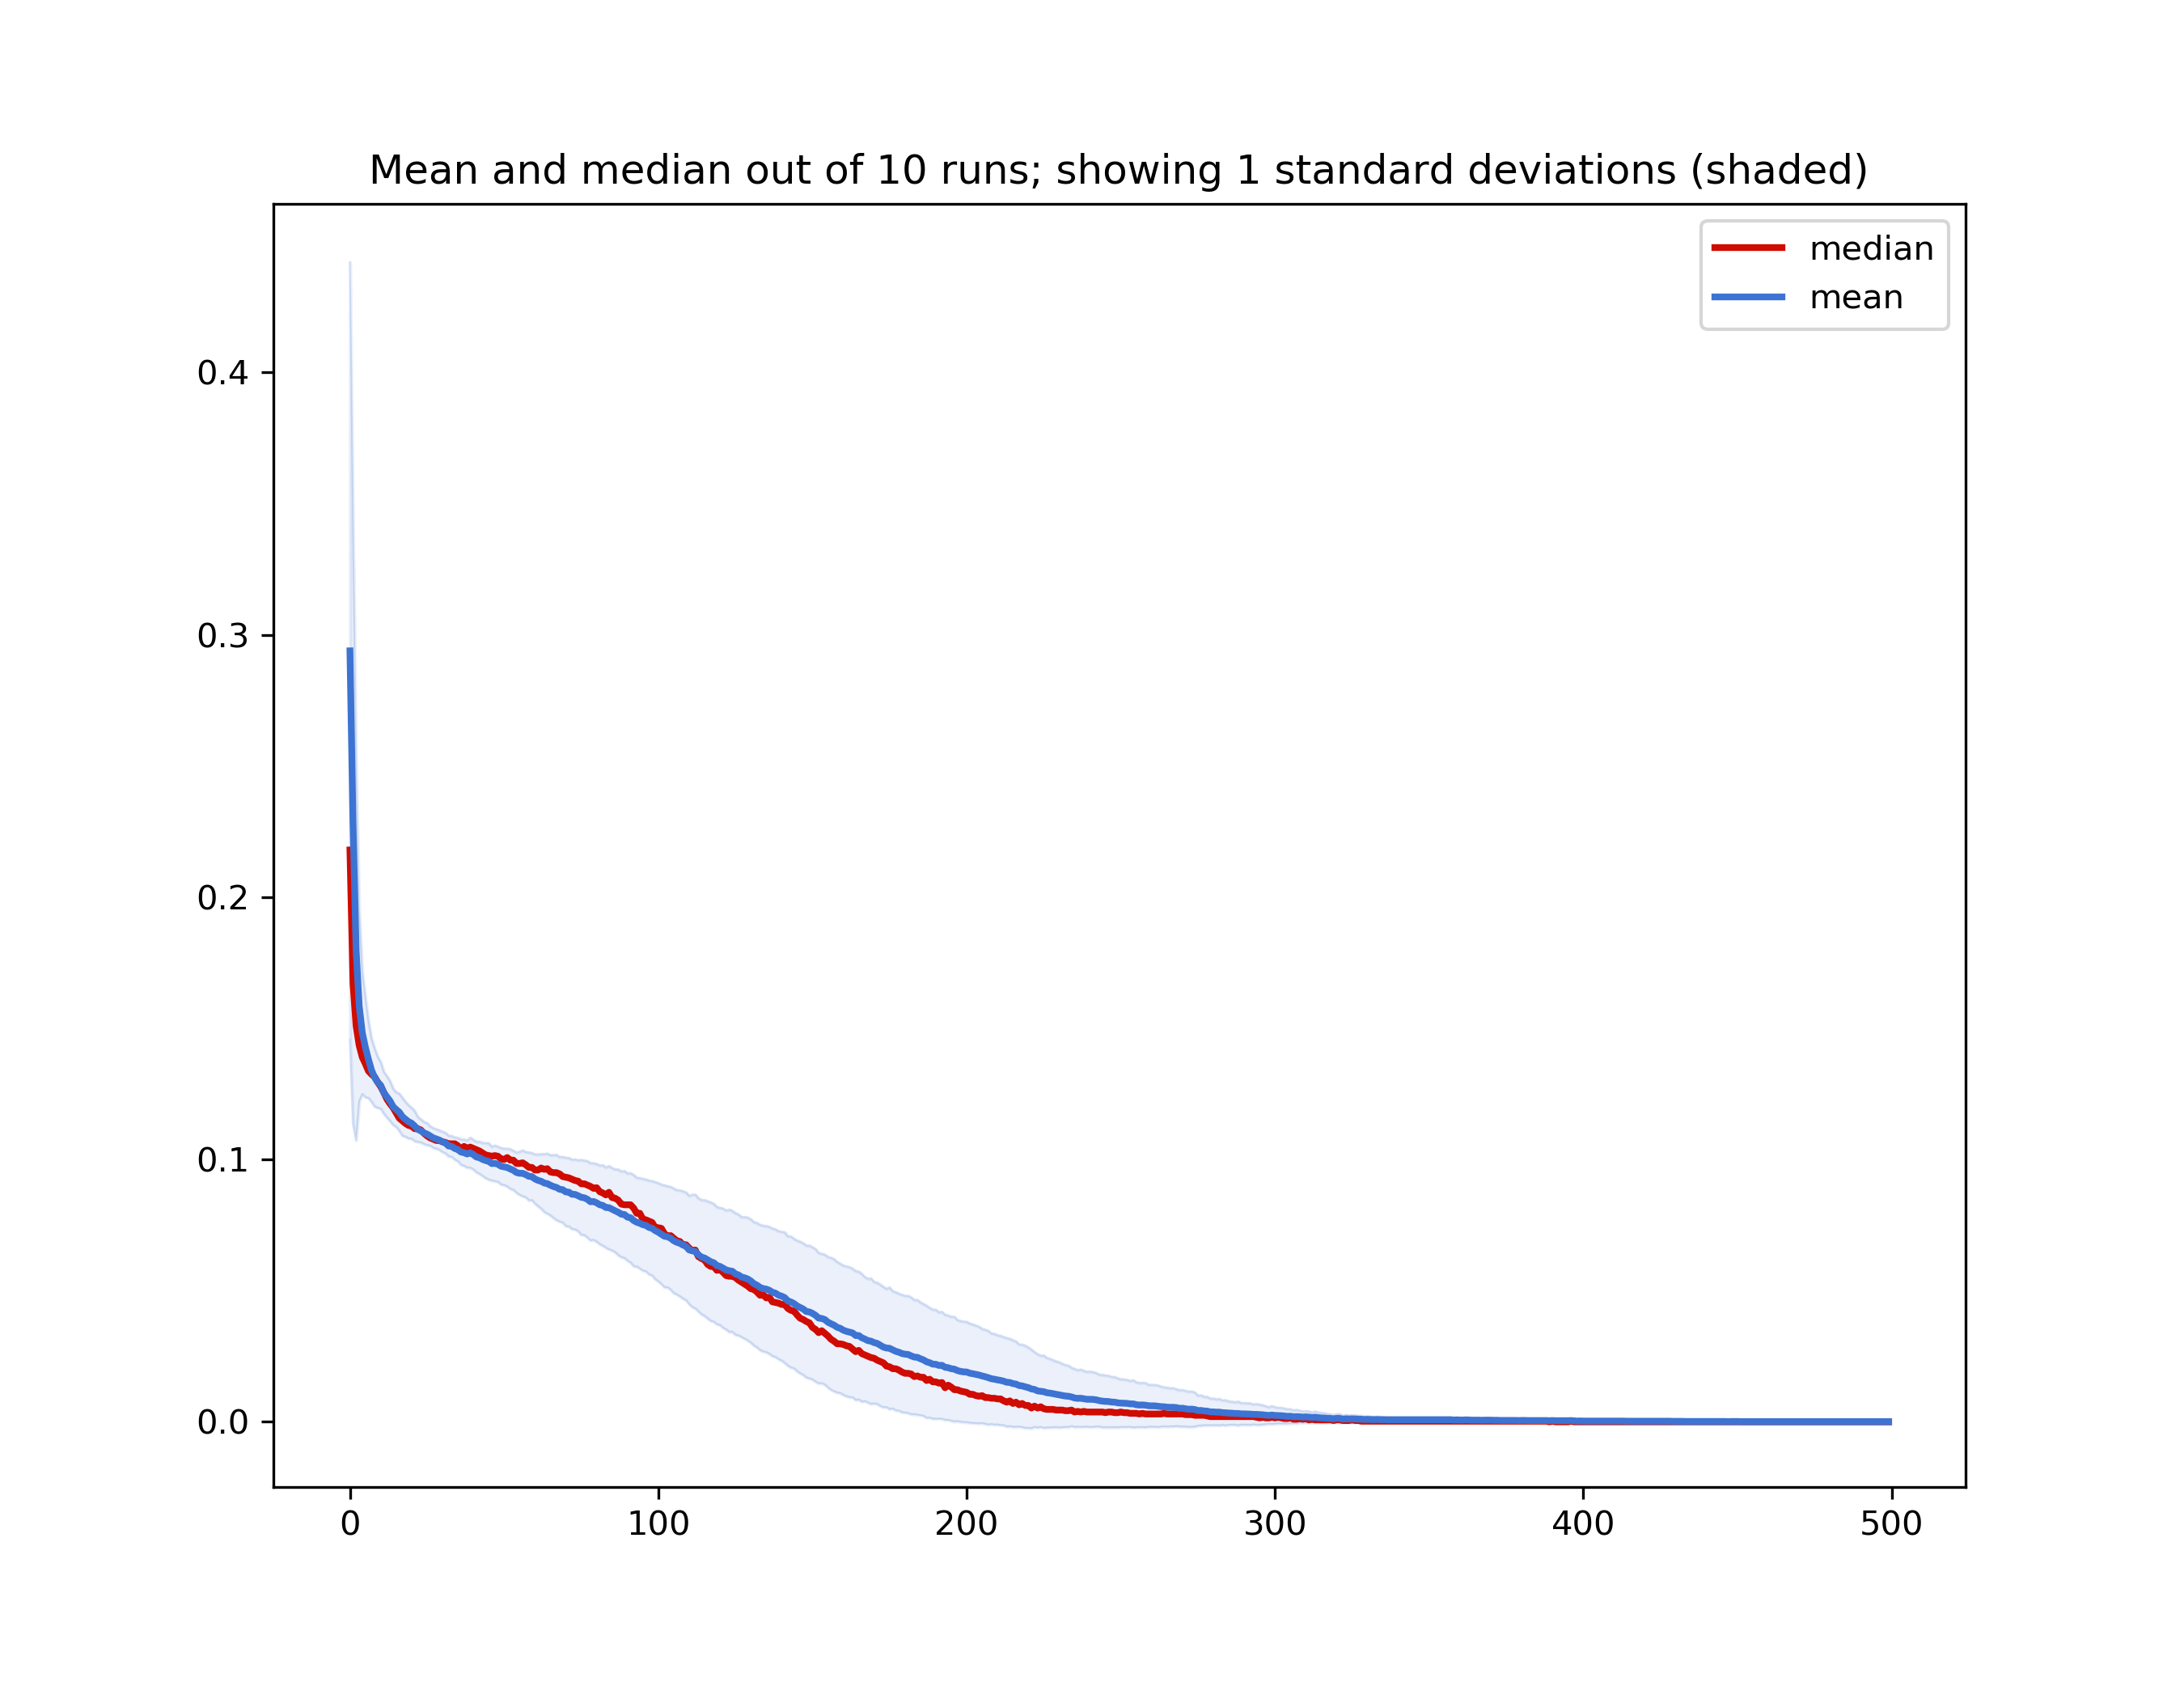
\includegraphics[scale=0.30]{pics/iv_ens}
	\caption{Training set error rate: mean and median with standard deviation; composed out of 10 runs.}
	\label{fig:iv_b}
	\end{subfigure}
\caption{Error rate on test set: $\gamma_t = 0.0$. NN is able to classify the system flawlessly.}
\label{fig:res_iv}
\end{figure}
\newpage
\noindent Additionally, it is worth mentioning that the NN is also able to classify other datasets, such as \texttt{sklearn.datasets.make\_circles} (see Figure \ref{fig:circ}) flawlessly.
\begin{figure}[h!]
\captionsetup[subfigure]{labelformat=empty}
\centering
	\begin{subfigure}{.48\textwidth}
	\centering
	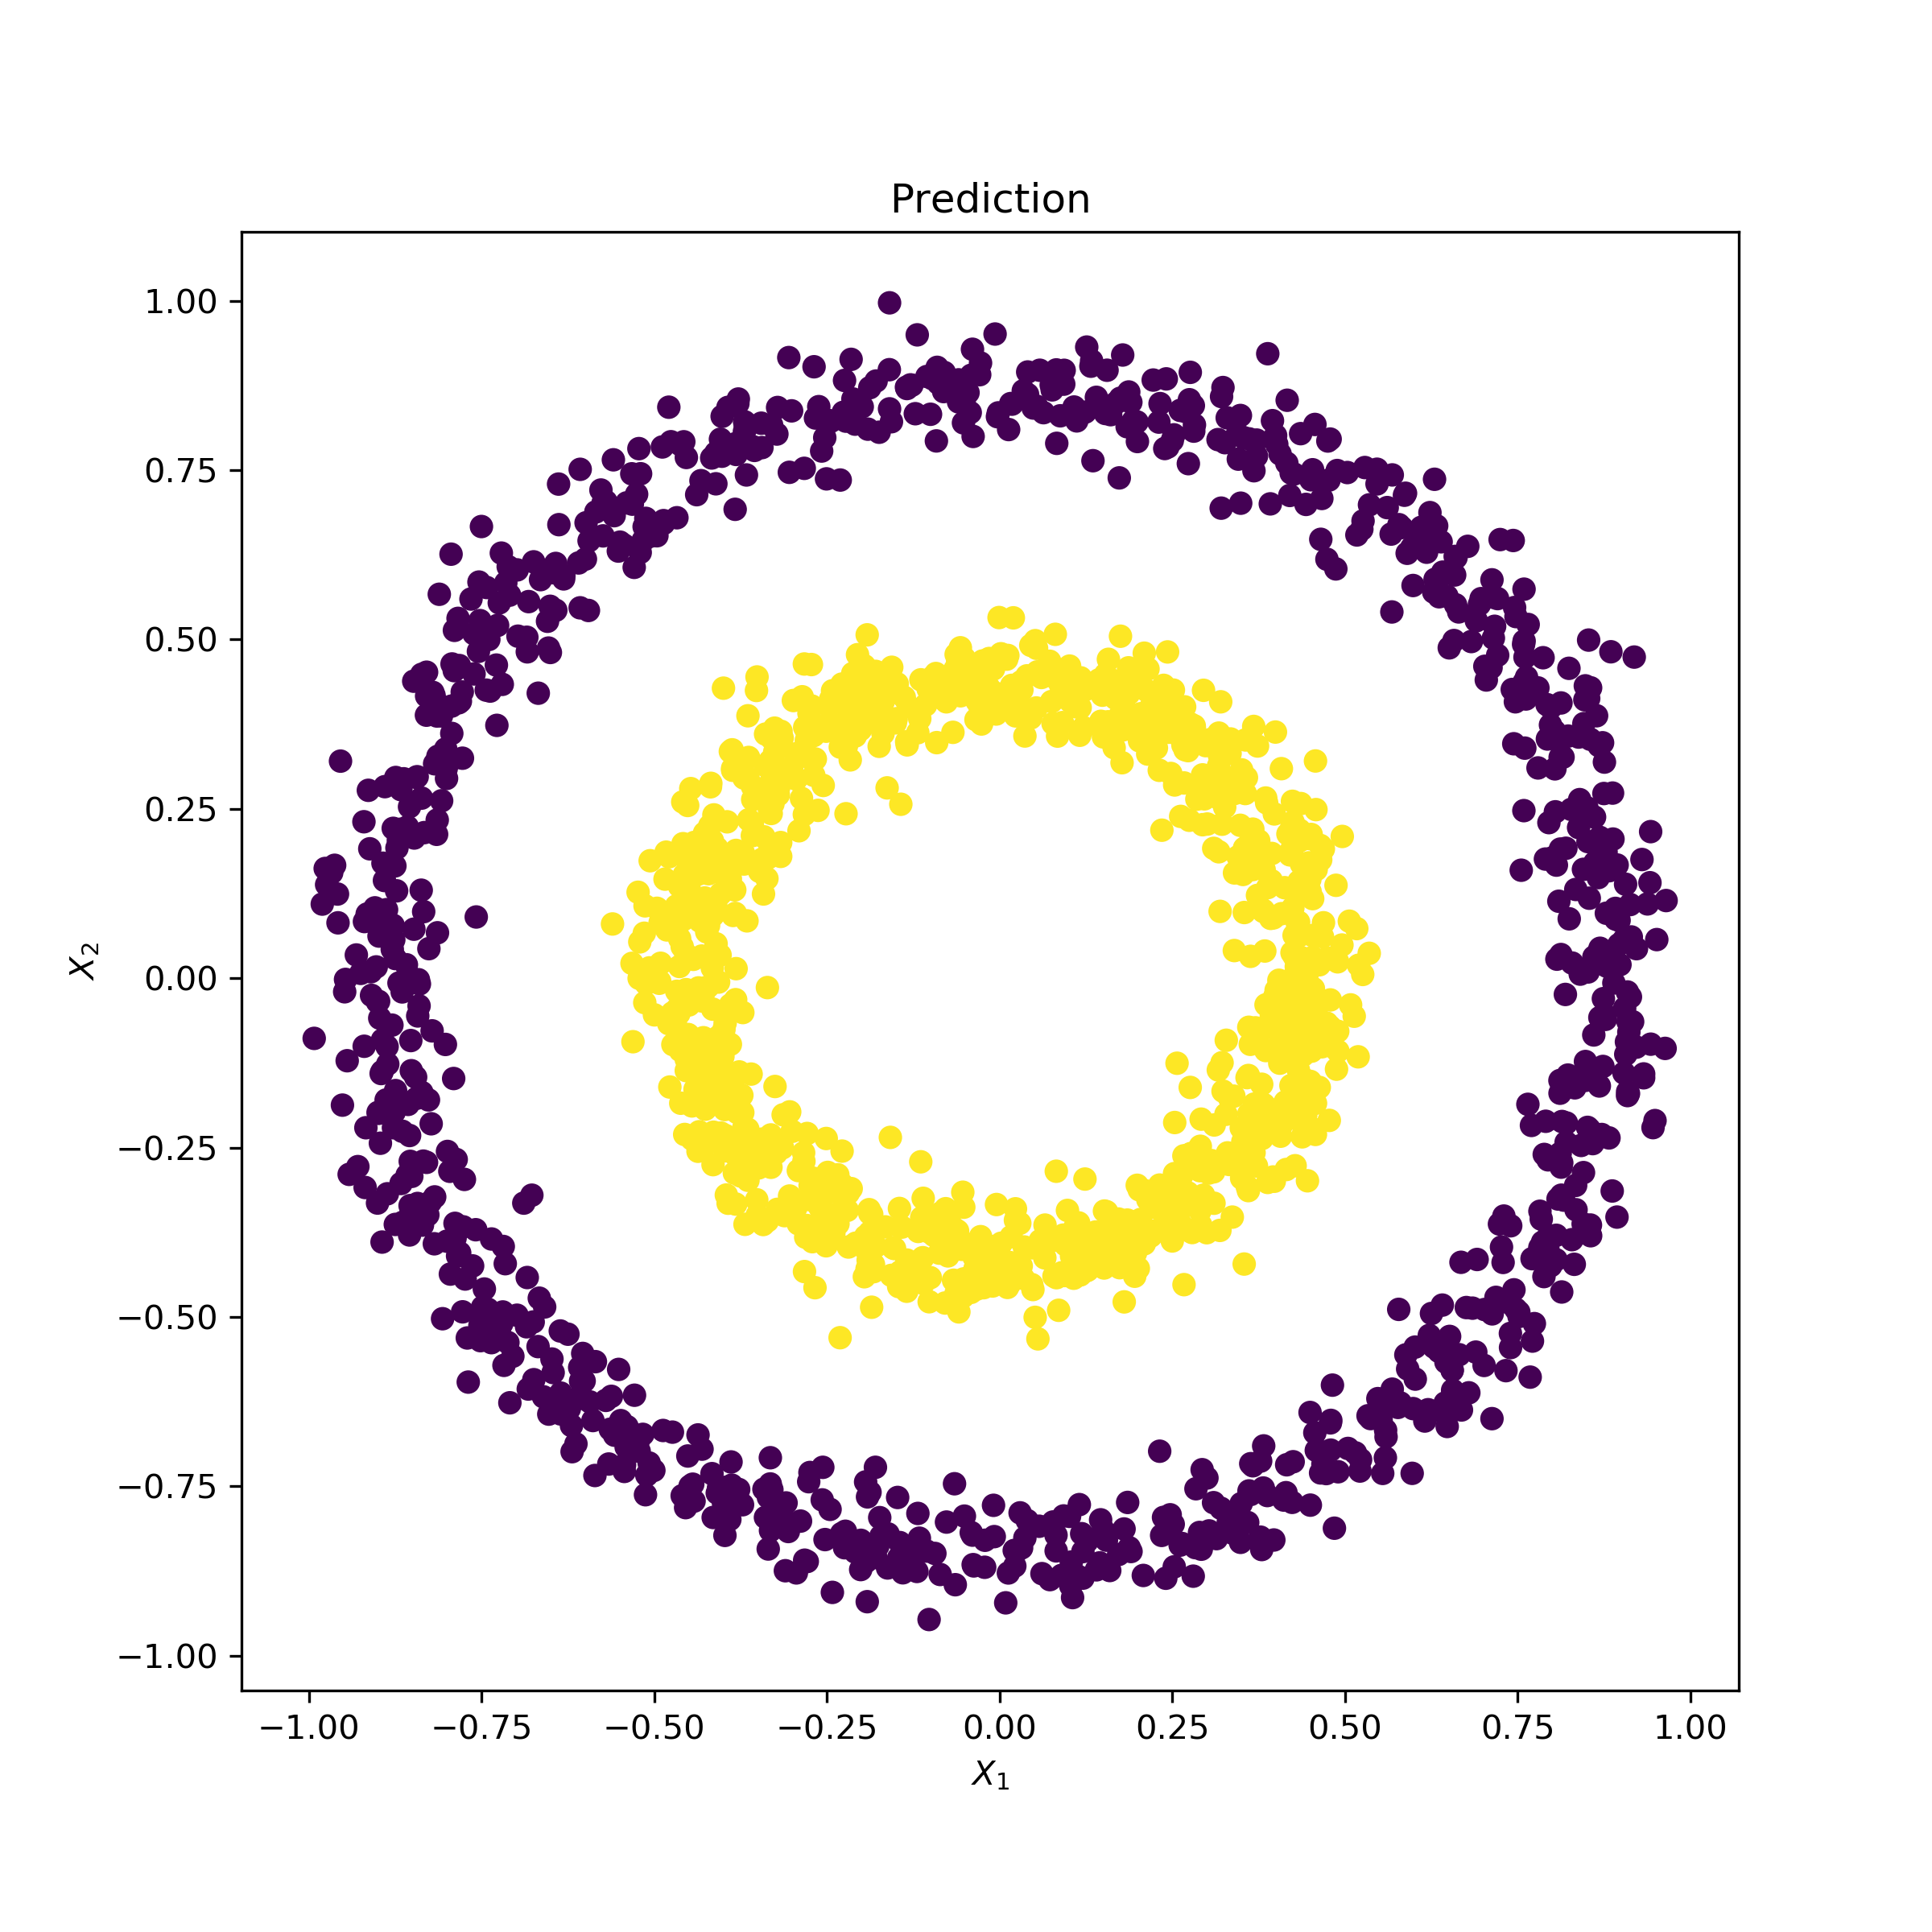
\includegraphics[scale=0.40]{pics/Prediction}
	\caption{Classification outcome on test set}
	\label{fig:v_a}
	\end{subfigure}
	\begin{subfigure}{.48\textwidth}
	\centering
	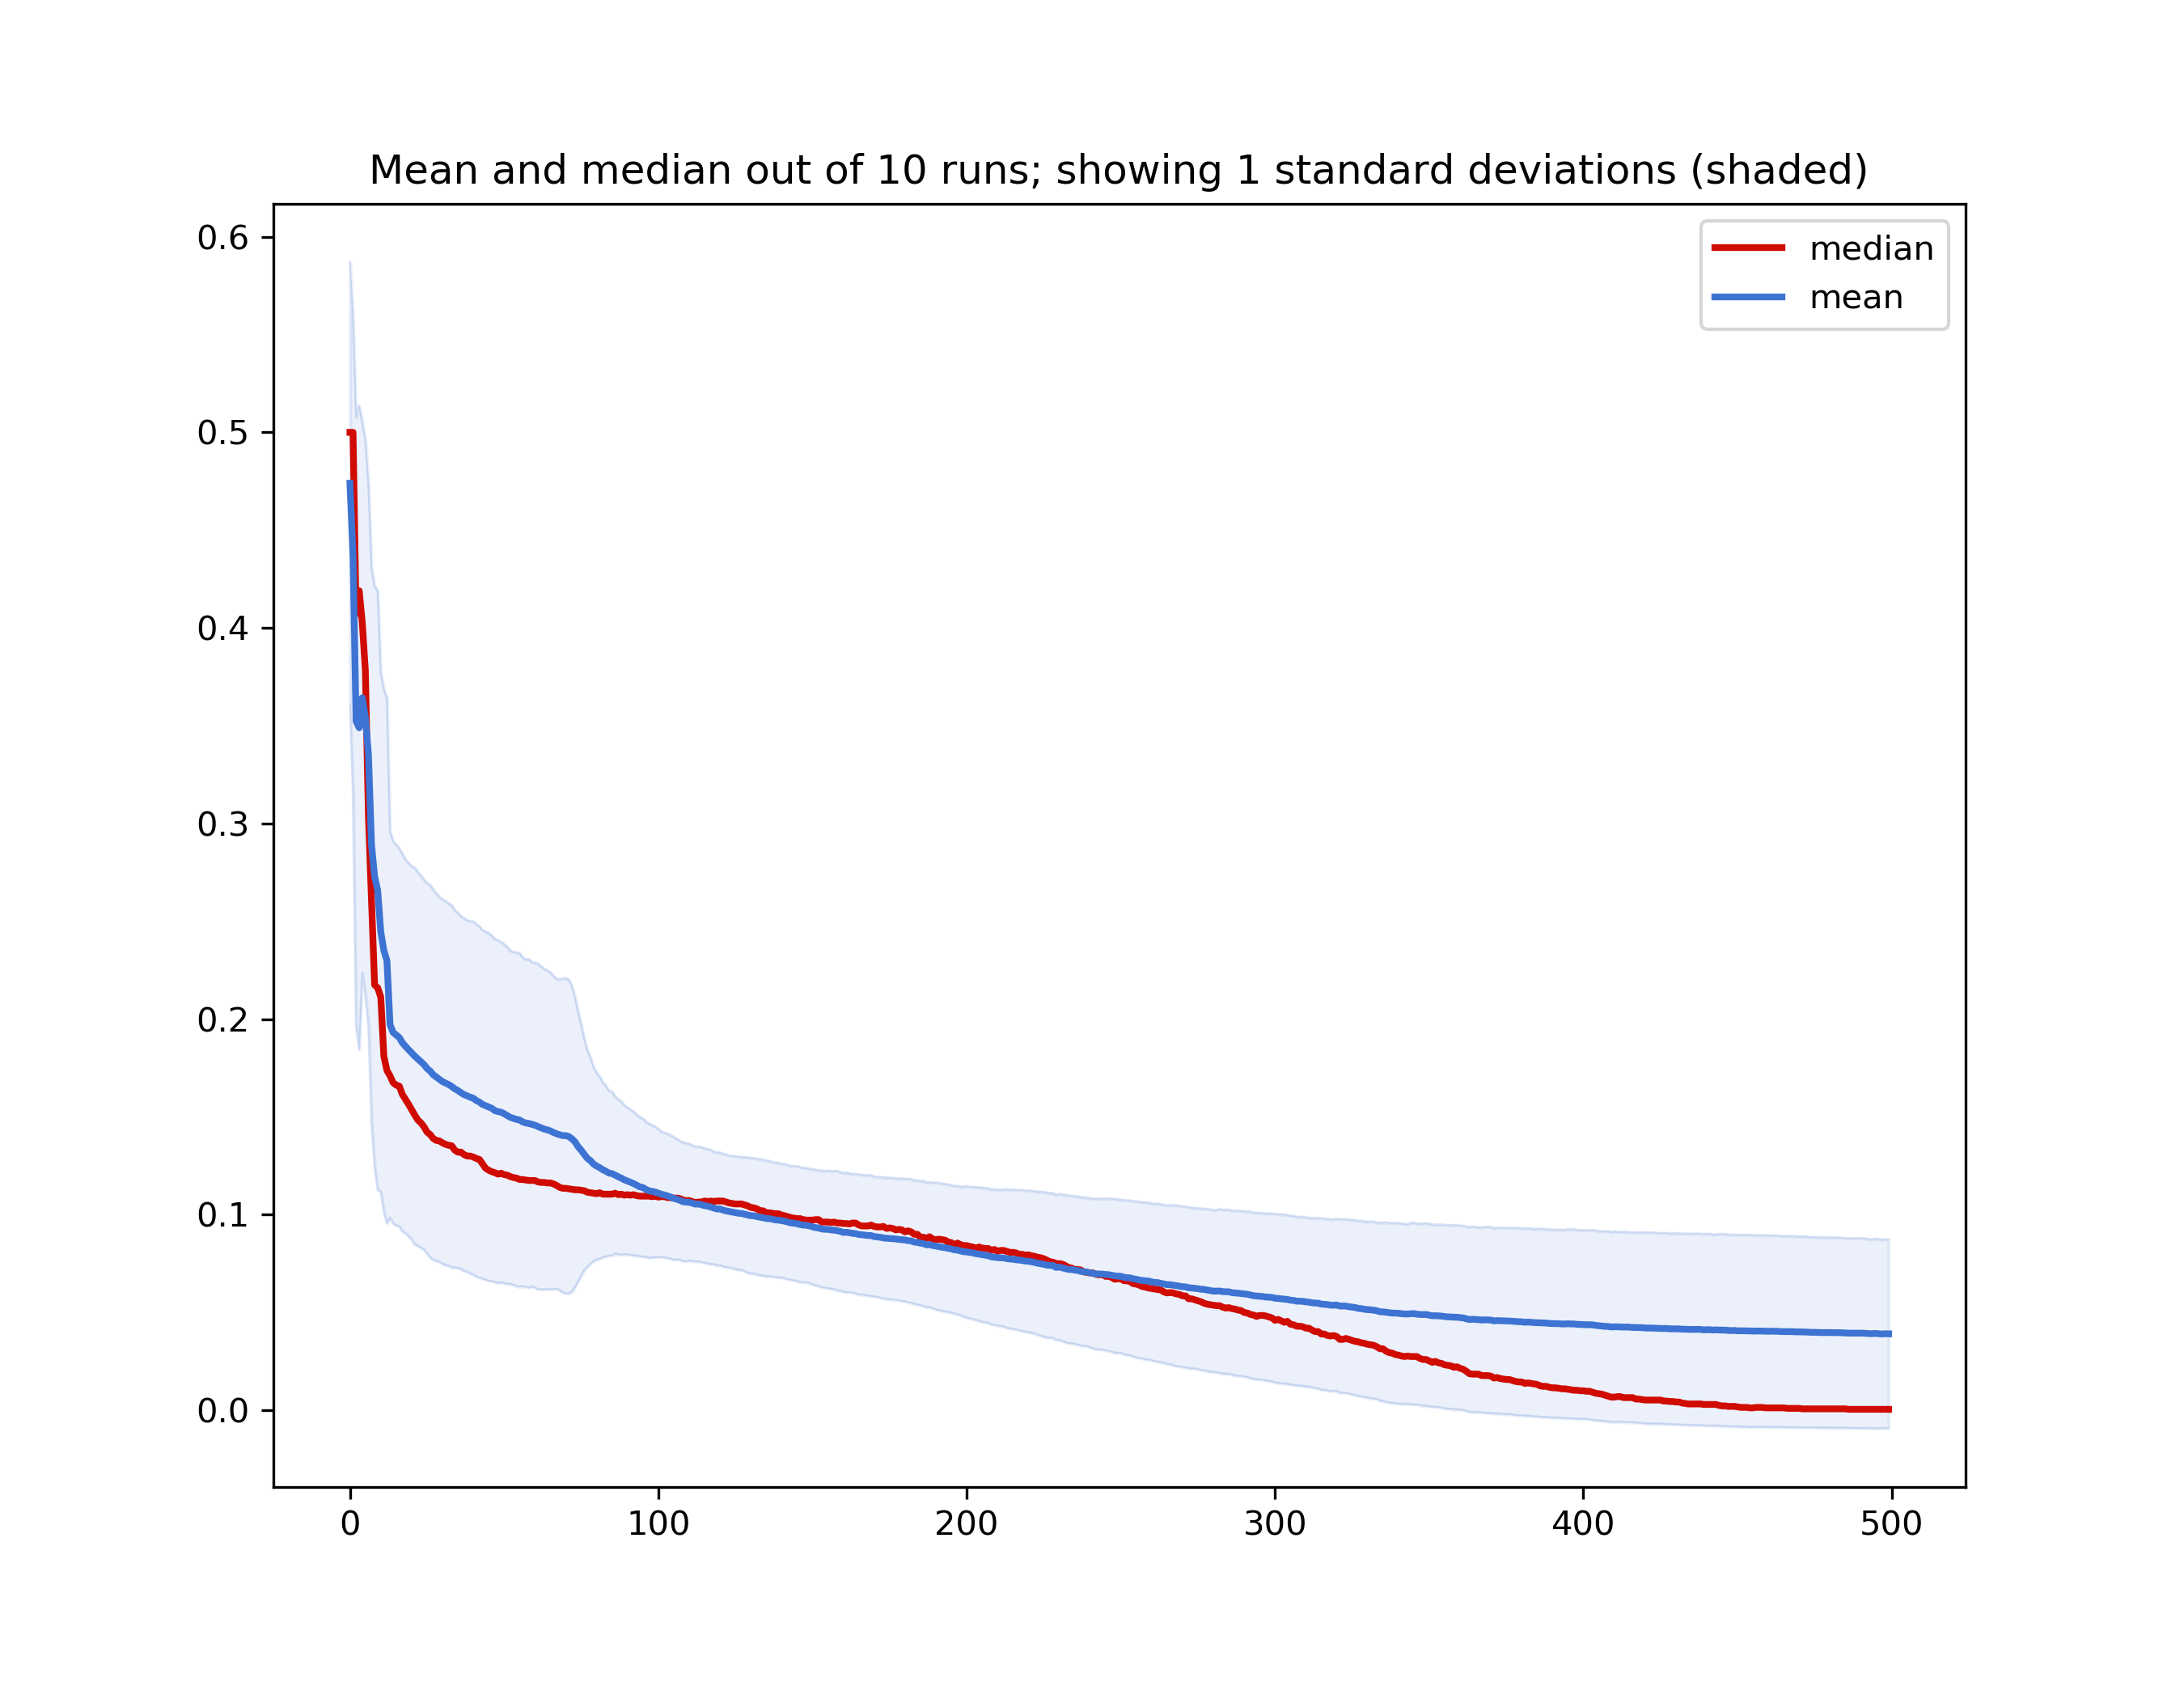
\includegraphics[scale=0.40]{pics/circle_ens_iii}
	\caption{Training set error rate: mean and median with standard deviation; composed out of 10 runs.}
	\label{fig:v_b}
	\end{subfigure}
\caption{\textsl{Circles} dataset. Error rate on test set: $\gamma_t = 0.0$. NN is able to classify the system flawlessly.}
\label{fig:circ}
\end{figure}

\end{document}
